\documentclass[12pt,english,brazil,a4paper,utf8,oneside]{utfpr-tcc}

% Este comando não é necessário: utilizei apenas para deixar o latex2rtf
% feliz (e descobrir a codificação do texto).
\usepackage[utf8]{inputenc}

% Suporte a figuras e subfiguras
\usepackage{graphics}
\usepackage{subfigure}

% Suporte a tabelas (principalmente do cronograma)
\usepackage{tabularx}
\usepackage{multirow}
\usepackage{array}
\usepackage{colortbl}
\usepackage{hhline}
\usepackage{xcolor}
\usepackage{indentfirst}
\usepackage{lscape}
\usepackage{appendix}

% Elementos geralmente utilizados na tabela do cronograma
\newcommand{\fullcell}{\multicolumn{1}{>{\columncolor[gray]{0.5}}c}{}}
\newcommand{\fullcellline}{\multicolumn{1}{>{\columncolor[gray]{0.5}}c|}{}}
\newcommand{\mc}[3]{\multicolumn{#1}{#2}{#3}}
\newcommand{\y}{\rule{8pt}{4pt}}
\newcommand{\n}{\hspace*{8pt}} 

% Define o caminho das figuras
\graphicspath{{images/}}

% Dados do curso que não precisam de alteração
\university{Universidade Tecnológica Federal do Paraná}
\universityen{Federal University of Technology -- Paraná}
\universityunit{Departamento Acadêmico de Computação}
\address{Campo Mourão}
\addressen{Campo Mourão, PR, Brazil}
\documenttype{Monografia}
\documenttypeen{Monograph}
\degreetype{Graduação}


%%%%%%%%%%%%%%%%%%%%%%%%%%%%%%%%%%%%%%%%%%%%%%%%%%%%%%%%%%%%%%%%%%%%%%%%%%%%%
% Alterar daqui para baixo
%%%%%%%%%%%%%%%%%%%%%%%%%%%%%%%%%%%%%%%%%%%%%%%%%%%%%%%%%%%%%%%%%%%%%%%%%%%%%

% Dados do curso. Caso seja BCC:
\program{Curso de Bacharelado em Ciência da Computação}
\programen{Undergradute Program in Computer Science}
\degree{Bacharel}
\degreearea{Ciência da Computação}

% Dados da disciplina. Escolha uma das opções e a descomente:
% TCC1:
%\goal{Proposta de Trabalho de Conclusão de Curso de Graduação}
%\course{Trabalho de Conclusão de Curso 1}
% TCC2:
\goal{Trabalho de Conclusão de Curso de graduação}
\course{Trabalho de Conclusão de Curso 2}


% Dados do TCC (precisa alterar)
\author{Emerson Yudi Nakashima}  % Seu nome
\title{Avaliação de atividades de programação submetidos em MOOC com emprego de técnicas de visualização} % Título do trabalho
\titleen{Evaluation of programming activities submitted in MOOC using visualization techniques} % Título traduzido para inglês
\advisor{Prof. Dr. Marco Aurélio Graciotto Silva} % Nome do orientador. Lembre-se de prefixar com "Prof. Dr.", "Profª. Drª.", "Prof. Me." ou "Profª. Me."}
\coadvisor{Profª. Drª. Aretha Barbosa Alencar} % Nome do coorientador, caso exista. Caso não exista, comente a linha.
\depositshortdate{2017} % Ano em que depositou este documento

% Dados da ficha catalografica. Ela é opcional, mas é uma boa ideia inserí-la. Exemplos para geração (http://fichacatalografica.sibi.ufrj.br/)
\fichacatautor{Nakashima, Emerson Y}  % Nome conforme citado (ou seja, no formato "Sobrenome, Nome").
\fichacatbib{Biblioteca da UTFPR de Campo Mourão} % Não alterar
\fichacatpum{N163} % Código Cutter-Sanborn. Use a primeira letra do sobrenome seguido do número conforme as primeiras letras do sobrenome e a tabela http://www.amormino.com.br/cutter-sanborn/cutter1.html
\fichacatpalcha{} % Assuntos do trabalho. Cada item deve ser enumerado e separado por ponto: 1. xxx. 2. yyy. 3. zzz.
\fichacatpdois{} % Deixar em branco


\begin{document}
	
\frontmatter
\maketitle

\begin{resumo}
\textbf{Contexto:} Em disciplinas de algoritmos ou programação, é necessário criar
e implementar uma solução para um problema. Entretanto, há a possibilidade de possuir
diversas formas de solucionar o problema e, consequentemente, formas de implementações.
Desta forma, a quantidade de implementações possíveis é vasta, dificultando a avaliação
delas pelo professor quanto ao custo, tempo e qualidade da avaliação.
Para agravar essa dificuldade, cursos massivos, abertos e \foreign{online} (MOOC)
possuem uma grande quantidade de usuários, inviabilizando
a correção individual das submissões.

\textbf{Objetivo:} O objetivo deste trabalho é propor subsídios para a avaliação de
programas submetidos em disciplinas introdutórias à computação, utilizando técnicas
de mineração e visualização de dados para construir e apresentar agrupamentos de
submissões semelhantes. Os subsídios propostos consistem na utilização de ferramentas
para extração de características, padronização no armazenamento dessas características
e a utilização de técnicas de agrupamento e visualização, com o auxílio de uma ferramenta.

\textbf{Método:} A primeira etapa consistiu na identificação das características que
podem ser extraídas conforme o tipo de análise utilizado: características estáticas
referentes a estilo de escrita e complexidade. Após a identificação, foi necessário
o desenvolvimento de ferramentas para coletar tais medidas de forma que pudéssemos
utilizá-las para realizar a projeção e visualização. Com isso, desenvolvemos uma
ferramenta para analisar as informações disponíveis, realizando os agrupamentos e
gerando uma visualização dos programas submetidos.
Para avaliar a visualização de submissões com auxílio da ferramenta, utilizamos
uma base de dados de implementações com soluções de cinco
problemas distintos. A avaliação ocorreu em duas etapas: mediante a qualidade
das visualizações, considerando as técnicas de mineração e visualização de dados; e
verificando o \foreign{feedback} da ferramenta para o professor por meio de um
questionário.

\textbf{Resultados:} Com uma base de dados de 152 implementações, obtivemos boa
avaliação da qualidade dos agrupamentos. Quanto à qualidade da visualização para
fins de avaliação das submissões, realizamos um treinamento com a apresentação
dos critérios de avaliação e da ferramenta. O estudo procedeu da utilização da
ferramenta \foreign{ScienceView}, criando uma nova base de dados, e dividindo
as correções em 2 grupos: um grupo realizara a correção tradicional e o outro
utilizara a ferramenta para auxiliar na correção. Em seguida, esses dois grupos
inverteram o modo como foi realizado as correções. Ao final do estudo,
os voluntários avaliaram o treinamento e a ferramenta positivamente.

\textbf{Conclusões:} 
Considerando a preservação de vizinhança, a qualidade da projeção é compatível
com outras projeções feitas com a técnica LSP e similares, apresentando resultados
similares relatados na literatura. Em relação ao emprego de visualização para
avaliação de programas, os resultados foram limitados devido ao emprego pouco
eficiente da ferramenta e dos agrupamentos. No entanto, considerando os agrupamentos
que continham programas avaliados, existem indícios de que a visualização pode
ser utilizada com êxito e, se melhorarmos o treinamento, poderemos alcançar
claramente nosso objetivo. Ainda assim, os participantes avaliaram como positiva
a utilização da ferramenta. Como trabalho futuro, serão investigadas a utilização
de outras características das submissões e o aperfeiçoamento da usabilidade e
treinamento quanto ao uso da ferramenta.

% Palavras-chaves, separadas por ponto (tente não definir mais do que cinco)
\vspace{.3cm}
\palavraschaves{MOOC. Programação. Avaliação. Agrupamentos. Mineração de dados. Visualização.}
\end{resumo}



% Caso seja TCC 2, precisa traduzir o resumo e as palavras-chaves para inglês:
\begin{abstract}
\textbf{Context:} In algorithm or programming classes, it is necessary to create and
implement a solution to a problem. However, there is the possibility of having several
ways so solve a problem and, consequently, forms of implementations. This, the amount
of possible implementations is vast, making it difficult for teachers to evaluate them
within reasonable cost, time and quality. Moreover,
massive courses, open and online (\acs{MOOC}) have large numbers of users, aggravating this
problem and making it unfeasible individual correction of submissions.

\textbf{Objective:} The objective of this project is evaluate and implement supporting tools
to assess programming assignments submitted in introductory courses to computing using
data mining and visualization techniques to build and show clusters of similar source codes. 

\textbf{Method:} The first step consisted of identification of features that can be
extracted according to static analysis and code style.
After this identification, we developed tools to colect such measures so
that we could use them for data mining and visualization. Thereby, we improved
an existing tool for performing clusters and generating visualizations of submitted
programming assingments. To evalute the tool, we have one collection of assignments'
submissions with solutions of 5 different
problems. The validation occurred in two steps: through the quality of the visualizations
considering the mining techniques and data visualization; and checking the feedback
of the tool by the teacher.

\textbf{Results:} With a database of 152 implementations, we obtained a good evaluation
of the quality of the clusters. Regarding the quality of the visualization for the purpose
of evaluating the submitted programs, we conducted an experimental study. The experimental
study was based on the use of the ScienceView tool, creating a new database, training the
study subjects with respect to the assessment criteria and tool, and assessing the
programming submissions. We organized the participants into two groups: one group
performed the traditional assessment and the other used the tool to aid in the assessment.
These two groups then switched how corrections were made. At the end of the experimental
study, the volunteers evaluated the training and the tool positively.

\textbf{Conclusions:} 
Considering the neighborhood preservation, the quality of the projection is compatible
with other projections made with the LSP technique and the like, presenting similar
results reported in the literature. In relation to the use of visualization for program
assessment, the results were limited due to the inefficient use of the tool and the
clusters. However, considering clusters containing programs evaluated by the experiment
participants, there are indications that visualization can be used successfully and, if
we improve training, we can clearly reach our goal. Nevertheless, the participants
assessed the use of the tool as positive. As future work, we will investigate the use
of other characteristics of the program and the improvement of usability and training
regarding the use of the tool.

% Palavras-chaves em inglês, separadas por ponto.
\vspace{.3cm}
\keywords{MOOC. Programming. Assessment. Clustering. Data mining. Visualization}
\end{abstract}


% Listas (opcionais, mas recomenda-se a partir de 5 elementos)
\listoffigures
\listoftables
\listofacronyms{acronimos}

% Sumário
\tableofcontents

\mainmatter
% TODO: incluir arquivos latex com os capítulos
\chapter{Introdução}

	\ac{MOOC} é uma plataforma de ensino online
	com cursos massivos e abertos que visa oferecer os mais diversos cursos a nível
	global. Para realizar um curso ofertado pelo \acs{MOOC}, é necessário apenas a conexão
	com a Internet e o cadastro na plataforma, geralmente gratuito. Foi popularizado
	em 2011 quando grandes universidades, como o Instituto de Tecnologia de
	Massachusetts, a Universidade de Harvard e a Universidade de Stanford tiveram
	a iniciativa mediados pelos provedores Cousera, edX e Udacity, respectivamente
	\cite{Mehlenbacher:2012}. Além de permitir explorar novos modelos de negócio
	\cite{dellarocas2013money}, possibilita englobar mais alunos a custos menores
	e com boa qualidade \cite{schmidt2013producing}.
	
	Em cursos de introdução a programação, seja \acs{MOOC} ou presencial, há uma introdução
	sobre algoritmo seguido da seleção de uma linguagem de programação para
	desenvolvimento. Alguns desses cursos orientam a utilização de ferramentas, como
	o \ac{IDE} e ensinam o funcionamento da linguagem sintaticamente.
	Entretanto, esse tipo de ensino tem levado o estudante a fazer seu programa baseado
	na tentativa e erro, visto que buscam gerar o algoritmo sem o total conhecimento
	lógico do problema \cite{edwards2003}. Isso funcionou como um incentivo para que
	surgissem outras abordagens de ensino, como a reflexão na ação (\foreign{Reflection
	in action}) e o \ac{TDD} \cite{camara_graciottoSilva2016}. Na primeira abordagem, a
	implementação do \foreign{software} ocorre somente após o entendimento apropriado
	do problema \cite{edwards2004}. No \acs{TDD}, cumpre-se um ciclo dividido em três etapas:
	na primeira etapa o programador insere um teste que deve falhar no momento de sua
	execução; na segunda etapa é implementado a solução para que o caso de teste
	escrito anteriormente seja aceito; e a última etapa refere-se a refatoração
	(simplificar ou melhorar) o código recém implementado \cite{beck2003}.
	
	Nesses cursos são necessários criar e implementar uma solução para um problema.
	Entretanto, há a possibilidade de possuir diversas formas de solucionar o problema
	e, consequentemente, formas de implementações. Desta forma, a quantidade de
	implementações possíveis é vasta, dificultando a avaliação delas pelo professor
	quanto ao custo, tempo e qualidade da avaliação. Além disso, é necessário realizar
	um \foreign{feedback} para o aluno com relação a sua implementação. Para agravar
	essa dificuldade, cursos massivos, abertos e \foreign{online} (MOOC) possuem uma
	grande quantidade de usuários, agravando este problema e inviabilizando a correção
	individual das submissões.

	Em cursos de introdução a programação, seja \acs{MOOC} ou presencial, há uma introdução
	sobre algoritmo seguido da seleção de uma linguagem de programação para
	desenvolvimento. Alguns desses cursos orientam a utilização de ferramentas, como
	o \ac{IDE} e ensinam o funcionamento da linguagem sintaticamente.
	Entretanto, esse tipo de ensino tem levado o estudante a fazer seu programa baseado
	na tentativa e erro, visto que buscam gerar o algoritmo sem o total conhecimento
	lógico do problema \cite{edwards2003}. Isso funcionou como um incentivo para que
	surgissem outras abordagens de ensino, como a reflexão na ação (\foreign{Reflection
	in action}) e o \ac{TDD} \cite{camara_graciottoSilva2016}. Na primeira abordagem, a
	implementação do \foreign{software} ocorre somente após o entendimento apropriado
	do problema \cite{edwards2004}. No \acs{TDD}, cumpre-se um ciclo dividido em três etapas:
	na primeira etapa o programador insere um teste que deve falhar no momento de sua
	execução; na segunda etapa é implementado a solução para que o caso de teste
	escrito anteriormente seja aceito; e a última etapa refere-se a refatoração
	(simplificar ou melhorar) o código recém implementado \cite{beck2003}.

\chapter{Referencial Teórico}
\label{chap:Ref}
	Neste capítulo serão apresentados os conceitos utilizados na pesquisa, bem como
	os estudos que fundamentaram esse projeto. A \cref{sec:Mooc} apresenta
	o conceito de MOOC e as principais características da plataforma de ensino.
	A \cref{sec:FundTeor} descreve as definições de termos presentes no
	decorrer da pesquisa: mineração, visualização, projeção, agrupamento e
	classificador. A \cref{sec:MinVisual} descreverá as características que
	podem ser extraídas dado a escolha de um dos tipos de análise de código-fonte.
	E a \cref{sec:TrabRel} apresenta as pesquisas relacionados a este estudo
	juntamente com suas limitações.

	\section{Massive Open Online Courses (MOOC)}
	\label{sec:Mooc}
		Após pesquisar o conceito de Curso Massivo, Aberto e \foreign{Online},
		\citeonline{fassbinder2014} observam que não há uma definição comum na
		literatura. Entretanto, encontra-se três descrições distintas para o termo.
		\citeonline{sivamuni2013} afirmam que o MOOC, em conformidade com o
		dicionário Oxford, é um curso oferecido por meio da Internet, de forma
		gratuita, para uma grande quantidade de alunos. \citeonline{subbian2013}
		reitera que o MOOC disponibiliza curso gratuito, baseado na \foreign{web},
		com registro livre de taxas monetárias e compartilhamento público de
		currículo. Por fim, \citeonline{siemens2013} defende a tendência em inovação e
		experimentação do uso da tecnologia para o ensino a distância e
		\foreign{online} a fim de dar oportunidade de aprendizagem de forma massiva.
		
		\citeonline{kim2014} afirma que massivo refere-se a capacidade do MOOC em
		suportar uma grande quantidade de alunos. Tal quantidade é bem superior
		ao número de discentes que uma sala pode acomodar ou o total de
		participantes em um curso \foreign{online} antes do surgimento do MOOC.
		Por exemplo, um curso de Inteligência Artificial foi ofertado, gratuitamente e
		\foreign{online}, pela Universidade de Stanford em 2011, no qual houveram
		160.000 estudantes inscritos \cite{rodriguez2012}.
		
		Entre os principais recursos da plataforma, como a integração com outras
		aplicações, como a utilização de e-mails e fóruns, o uso de questionário
		relacionados com os vídeos e a inclusão de atividades para estimular e
		motivar os alunos \cite{fassbinder2014}. Focaremos no desenvolvimento de
		recursos avançados de visualização dos dados obtidos por meio das
		implementações submetidas em cursos de programação e na realização de
		\foreign{feedback} para que o usuário possa verificar seu nível de conhecimento.

	\section{Mineração e Visualização de Dados}
	\label{sec:FundTeor}
		Nesta seção apresentaremos as definições de alguns termos utilizados
		durante a pesquisa: mineração, a diferença na área de Inteligência
		Artificial sobre classificadores e agrupamento, visualização de dados e projeção.

		\begin{figure}[h]
			\centering
			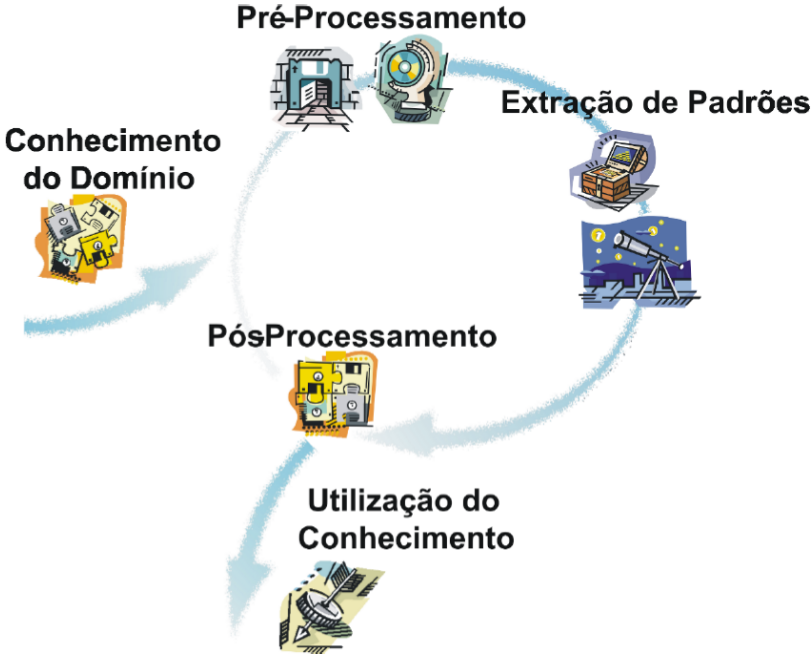
\includegraphics[width=0.7\linewidth]{imagem/mineracaoDados}
			\captionsetup{justification=centering}
			\caption{Etapas da mineração de dados \cite{rezende2003}}
			\label{fig:mineracaoDados}
		\end{figure}
		
		A mineração de dados é uma etapa do \foreign{Knowledge Discovery in Databases}
		\cite{fayyad1996} que busca descobrir padrões em grandes conjuntos de dados
		podendo utilizar métodos de inteligência artificial, estatísticos e sistemas
		de banco de dados \cite{chakrabarti2006}. O objeto do processo de mineração
		de dados consiste na extração de informações de um conjunto de dados e
		transformá-lo em uma estrutura compreensível para uso posterior \cite{chakrabarti2006}.
		A \cref{fig:mineracaoDados} apresenta os estágios da mineração de dados:
		o Conhecimento do Domínio condiz com a identificação do problema para possuir
		um conhecimento inicial e, definir as metas e os objetivos a setem atingidos
		no processo de extração de conhecimento; a etapa Pré-processamento refere-se
		a padronização e limpeza da extração de dados de fontes diversas e, a escolha
		de um subconjunto representativo; a fase seguinte, Extração de Padrões, 
		consiste na aplicação do algoritmo de mineração de dados escolhido; o estágio
		Pós-processamento equivale a análise dos padrões obtidos anteriormente e
		possibilita a extração de outros padrões; por fim, a Utilização do Conhecimento
		é a utilização dos dados extraídos em algum sistema ou utilizado diretamente
		pelo usuário. Muitos métodos de mineração de dados são baseados em técnicas de treinamento
		e teste de aprendizagem de máquina e, reconhecimento de padrões e estatísticas,
		como os algoritmos de classificação e agrupamentos, respectivamente \cite{fayyad1996}.
		
		Classificação é a tarefa de aprendizagem de uma função alvo que mapeia cada
		conjunto de atributos a um dos rótulos de classe predefinidas \cite{Tan:2005:ch4}.
		Uma função alvo auxilia como uma ferramenta que possui informações para distinguir
		os objetos de diferentes classes. A fim de realizar essas classificações, são
		implementados classificadores com diversas abordagens, como árvores de decisão,
		redes neurais e \foreign{support vector machine}, por exemplo. Esses
		classificadores são mais utilizados para predizer ou descrever um conjunto
		de dados com categorias binárias ou nominais \cite{Tan:2005:ch4}. Por exemplo,
		para classificar um animal como mamífero, réptil, peixe, anfíbio ou pássaro,
		deve-se sumarizar dados como a temperatura do corpo, característica da pele,
		se é uma criatura aquática, se possui patas e hiberna.
		
		O que difere a classificação do agrupamento, é que esse é formado por meio da
		comparação de informações entre os objetos e não existem rótulos pré-definidos,
		enquanto aquele é realizado por meio da comparação das informações do objeto
		com os dados contidos na função alvo. Desta forma, os objetos dentro de um grupo
		devem ser similares ou relacionados entre si e, diferentes ou não relacionados
		entre objetos de grupos diferentes, ou seja, quanto maior a similaridade dos
		objetos dentro de um grupo e mais diferentes são os agrupamentos, melhor ou
		mais distinto os agrupamentos \cite{Tan:2005:ch8}. O K-means \cite{macqueen1967}
		e o \foreign{Density-based Algorithm for Discovering Clusters} \cite{Ester1996}
		são exemplos de algoritmos de agrupamento.

		Após a mineração dos dados, é desejável a utilização de ferramentas para
		auxiliar na criação de hipóteses sobre conjuntos de dados complexos -- grande
		conjunto de dados ou de alta dimensionalidade -- para que os analistas possuam
		capacidade de explorá-los e compreendê-los \cite{de2003}. A visualização de dados
		produz modelos gráficos e representações visuais a fim de utilizar a capacidade
		cognitiva do ser humano, por meio da percepção visual, para colaborar com
		a exploração e obtenção de informações úteis presente nos dados \cite{de2003,keim2002}.
		Ademais, a visualização de dados é intuitiva, permitindo explorar os dados
		mais rápido e fornecendo melhores resultados na maioria das vezes \cite{keim2002}.
		
		Entretanto, não é possível gerar visualizações sobre conjuntos de dados
		complexos. Assim sendo, é necessário a utilização de técnicas de projeção que
		criam o mapeamento de dados para reconhecimento visual \cite{friedman1974} e,
		com isso, produzir a visualização. Devido a alta dimensionalidade dos dados,
		é necessário a utilização de projeções multidimensionais. Essa técnica realiza
		a diminuição $n-dimensional$, sendo $n$ uma alta dimensão, para uma espaço
		unidimensional, bidimensional ou tridimensional \cite{paulovich2008least}.
		Para criar essa visualização deve-se selecionar o formato de como as
		características extraídas serão armazenadas, como o vetor de características
		ou o modelo de tabela de dados \cite{de2003}.

	\section{Mineração e Visualização de Programas}
	\label{sec:MinVisual}
		Para realizar a mineração de informações nos programas submetidos, é necessário
		decidir como serão extraídos as características -- análise sintática, dinâmica e
		do código de escrita -- e quais dados podem ser obtidos por meio da análise
		escolhida (\cref{subSec:Caracteristicas}). Independente da dimensão
		obtida por meio da quantidade de informações extraídas, é necessário escolher
		como os dados obtidos serão representados para que seja possível realizar sua visualização.
		
		\subsection{Características de Programas}
		\label{subSec:Caracteristicas}

			A extração de características por meio das implementações podem ocorrer das
			seguintes formas: análise estática, análise dinâmica e análise do estilo de escrita.
			A análise estática ocorre por meio da observação do código-fonte, considerando
			apenas sua implementação, ou seja, não é necessário sua execução. Há diversas
			características que podem ser extraídas dessa análise. Há abordagens que extraem
			somente a Árvore de Sintaxe Abstrata (AST) que pode ser gerada durante a análise
			sintática do compilador para representar o código-fonte em forma de árvore
			armazenando símbolos não-terminais nos nós filhos e símbolos terminais nos
			nós folha, como representa a \cref{fig:AST} em uma declaração de condição.
			Esse tipo de árvore possui símbolos não terminais como nós filhos
			e símbolos terminais como nós folhas. Enquanto outras abordagens extraem
			características como: a quantidade de linhas e atribuições da implementação,
			a complexidade ciclomática \cite{mccabe}, quantidade de variáveis, operadores,
			operandos, laços de repetição e laços de repetição aninhados, por exemplo.
						
			\begin{figure}[h]
				\centering
				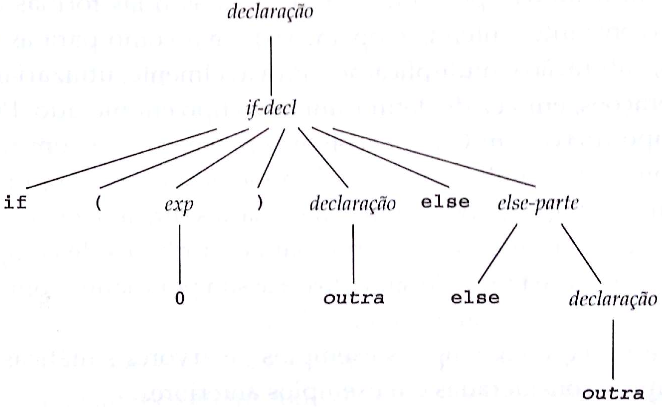
\includegraphics[width=0.7\linewidth]{imagem/AST}
				\captionsetup{justification=centering}
				\caption{Representação de árvore de sintaxe abstrata \cite{louden2004}.}
				\label{fig:AST}
			\end{figure}
			
			A análise dinâmica do código-fonte consiste na observação da execução do
			programa, por meio do \foreign{trace} -- uma espécie de histórico de execução
			do programa -- e de teste de \foreign{software}. Analisando esse histórico é
			possível verificar algumas características, como: em que momento foi realizado
			uma atribuição, chamada de função e recursão, qual bloco de código foi
			executado em uma declaração de condição, a quantidade de vezes que um laço
			de repetição foi executado e a saída no final da execução. Já o teste de
			software pode ser utilizado executando casos de teste nos quais é verificado
			se produção final do programa era o esperado e esta informação, se o caso de
			teste funcionou corretamente ou não, também pode ser uma característica do programa.
			
			E a análise do estilo de escrita, que será utilizada no desenvolvimento desse projeto,
			é um tipo da análise estática. Entretanto, se difere no fato das implementações estarem
			sintaticamente corretas. Nesse tipo de análise é considerado o estilo de escrita do
			programador, abrindo a possibilidade de coletar dado estáticos, como a quantidade de
			linhas de código e sua complexidade. Além da possibilidade de coletar
			características da análise estática citada anteriormente, é possível coletar se:
			há mais que uma instrução e importação de bibliotecas por linha, há espaços entre
			operando e operador, os métodos são separados por uma linha em branco e tamanho
			da instrução, medido em caracteres. A \cref{tab:exemploEstEsc} exemplifica
			possíveis características de serem extraídas em uma chamada de função, na qual é
			possível inserir ou não um espaço entre o parâmetro e os \foreign{tokens} abrir
			e fechar parêntese, como também a utilização de uma ou mais instruções por linha.
			
			\begin{table}
				\centering
				\begin{tabular}{|c|c|}
					\hline
					Chamada de função & Instrução por linha \\ \hline
					primo(7)          & a = 5 * 3  \\
					primo( 7)         & primo(7)     \\
					primo(7 )         &      \\
					primo( 7 )        & a = 5 * 3; primo(7)    \\
					\hline
				\end{tabular}
				\captionsetup{justification=centering}
				\caption[Representação do estilo de escrita]{Representação do estilo
				de escrita em uma chamada de função e instrução por linha.}
				\label{tab:exemploEstEsc}
			\end{table}
			
			Além da possibilidade de extrair os dados citados anteriormente. É possível
			obter os dados de como foi realizado o processo técnico e social do desenvolvimento
			do programa. Para ambas abordagens, é necessário a utilização de um sistema de
			controle de versão para que se possa utilizar seus recursos. Um mecanismo para
			obter informações é em relação ao momento, data e hora, em que o aluno realizou
			um \foreign{commit} de uma versão da sua implementação. Outro método é verificar
			se houve comunicações com outras pessoas durante o desenvolvimento do programa,
			por meio da interação em \foreign{issues} ou solicitações de \foreign{pull requests}.
			
			\textbf{Eu não entendi a seguinte inserção nessa subseção que você solicitou:
				"Problema (atividade de aprendizagem sendo elaborada)"}

	\section{Trabalhos Relacionados}
	\label{sec:TrabRel}
	
	    A fim de encontrar a semelhança entre os códigos, \citeonline{Yin:2015}
	    utilizou a AST. Após a criação das árvores, é necessário o uso de métricas
	    para verificar a similaridade entre as árvores. Desta forma, foi utilizada
	    a Distância de Edição de Árvore (TED) – ao comparar duas árvores, verificam-se
	    quais são as movimentações (inserção, movimentação e remoção) necessárias
	    para que as árvores fiquem iguais. Assim, foi selecionada a TED normalizada
	    que utiliza estrutura \foreign{top-down}: quanto mais próximo do nó raiz,
	    maior sua importância. Sua escolha ocorreu pelo fato da TED normalizada
	    possuir maior índice na qualidade de agrupamentos.
	    
	    Os autores desse artigo utilizaram os algoritmos de agrupamento
	    DBSCAN \cite{Ester1996} e OPTICS \cite{Ankerst1999} para agrupar os códigos
	    semelhantes. Tais algoritmos foram selecionados devido a maior pontuação
	    de silhueta. Essa pontuação verifica a similaridade entre pares dentro do
	    agrupamento e entre os agrupamentos. Quanto maior sua pontuação, melhor a
	    qualidade do \foreign{cluster}. Conforme a \cref{fig:t-SNE}, para
	    visualizar os agrupamentos foi utilizado o t-SNE \cite{maaten2008} – técnica
	    utilizada para reduzir dados de alta dimensionalidade para duas ou três
	    dimensões preservando a estrutura local dos dados.
	    
	    \begin{figure}[ht]
	        \centering
	        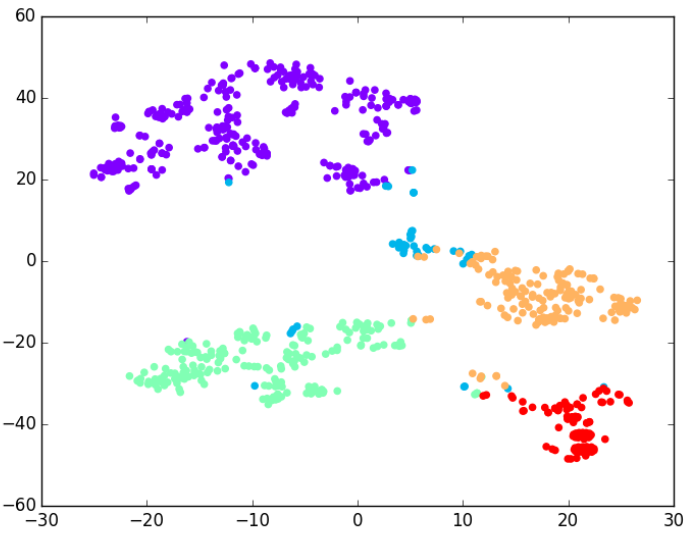
\includegraphics[scale=0.5]{imagem/visualizacao-tSNE.png}
	        \captionsetup{justification=centering}
	        \caption{Visualização t-SNE \cite{Yin:2015}}
	        \label{fig:t-SNE}
	    \end{figure}
	    
	    \textbf{Professora, na primeira revisão você questionou o que a função
	    	combine\_anagrams faz. Entretanto, revisei o artigo e não é realizado
	    	nenhuma menção ao objetivo da função. Devo tirar o nome da função? E
	    	a figura citada abaixo estava aqui! rs}
	    
	    Na \cref{fig:t-SNE} é possível observar cinco grupos distintos
	    criados a partir da comparação das TEDs normalizadas destacados em cores
	    diferentes. Cada ponto presente na visualização corresponde a uma
	    implementação. Todas as implementações possuem a função \foreign{combine\_anagrams}
	    que possui a variável \foreign{words} como parâmetro: no grupo vermelho,
	    essa função possui 3,7 linhas; no agrupamento roxo, 10,9 linhas; no
	    grupo laranja, a função possui 12,5 linhas; e no agrupamento verde,
	    a solução possui 21,3 linhas. Enquanto os pontos azuis não obtiveram
	    similaridade suficiente para formar um agrupamento ou serem classificados
	    em outro agrupamento, ou seja, \foreign{outliers}. 

		A extração de características por meio da AST é interessante, como também
		o uso da TED normalizada para verificar sua similaridade, devido ao seu
		baixo custo computacional. Entretanto, como o autor testou seu agrupamento
		somente com implementações para resolver um único problema, não sabemos se
		tal abordagem é eficiente quando houver implementações que buscam resolver
		diversos problemas. Em razão da possibilidade dos códigos-fontes gerarem
		árvores parecidas ainda quando solucionam problemas distintos.
	    
	    Em \citeonline{Glassman:2014}, foi proposto um agrupamento hierárquico de dois
	    níveis. No nível mais alto ocorre o particionamento das soluções ao longo do
	    plano de separação, considerando apenas características abstratas, como, por
	    exemplo: posição da declaração de condicional em relação a declarações de laço
	    de repetição (antes, dentro ou depois), profundidade de um laço de repetição
	    (\foreign{loop}) aninhado, números de nós AST e declarações de retorno,
	    \foreign{loops} e comparações, por exemplo.
	    
	    Dentro de cada agrupamento de alto nível, existem subagrupamentos internos,
	    destinado a capturar a dimensão generalizada, construções de linguagem de
	    baixo nível e bibliotecas utilizadas. Os agrupamentos internos são formados
	    por meio de 48 características concretas: operações aritméticas e lógicas,
	    laços de repetição, funções de bibliotecas, declarações de atribuição,
	    \foreign{loops}, condicional, número de variáveis e valores constantes,
	    por exemplo.
	    
	    \citeonline{Glassman:2014} utilizam o algoritmo de agrupamento \foreign{K-means}
	    para agrupar as implementações dos estudante. Foram utilizados diversos valores
	    para $k$ e a validação dos agrupamentos ocorreu por meio da comparação dos
	    \foreign{clusters} criado pelo algoritmo de classificação com o que foi criado
	    pelos professores. Para os professores foram entregues 50 códigos dos estudantes
	    randomicamente distribuídos e notou-se que eles ignoraram características de baixo nível.
	    
	    Estes utilizaram a métrica Informação Mútua Ajustada (AMI, do inglês
	    \foreign{Adjusted Mutual Information}), cálculo probabilístico, para comparar
	    os agrupamentos dos professores com cada agrupamento gerado pelo \foreign{k-means}.
	    Quando o valor de AMI é 0 (zero), quer dizer que os agrupamentos são
	    independentes, entretanto, se for igual a 1, indica perfeita concordância
	    entre os \foreign{clusters}. Quando $k$ tinha um valor maior ou igual a 15,
	    os agrupamentos concordaram com o agrupamento de cada professor, conforme
	    medição do AMI.
	    
	    Apesar da grande quantidade de dados extraídos das implementações, não houve
	    nenhum alusão sobre como essas características interfeririam na cálculo de
	    similaridade utilizada. Contudo a abordagem de dividir as informações a serem
	    coletadas em duas dimensões é relevante. Posto que as implementações com
	    a mesma quantidade de laços de repetição, por exemplo, deveriam ser agrupadas
	    facilitando a verificação se os alunos entenderam como fazer e utilizar
	    tal instrução.
	    
	    Em \citeonline{Taherkhani:2012}, testou-se a ferramenta Aari para cinco tipos
	    de métodos de ordenação: \foreign{bubble sort}, \foreign{insertion sort},
	    \foreign{selection sort}, \foreign{mergesort} e \foreign{quicksort}. Os autores
		separaram as características em quatro categorias: características numéricas,
		características descritivas, características de algoritmos de ordenação e
		outras características.
	    
	    A categoria de características numéricas extrai tudo que pode ser medido
	    como inteiro e possui o seguinte conjunto de características: número de
	    declarações de atribuição; número de linhas de código; complexidade McCabe;
		total de operadores; total de operandos; número de operadores único; número
		de operando único; total do número de operadores e operandos; total do número
		de operadores e operandos únicos; número de variáveis; número de laços de
	    repetição; número de laços aninhados e número de bloco.
	    
	    A categoria de características descritivas possui: se um algoritmo é
	    recursivo, se é uma recursão em cauda, regras de variáveis e \foreign{arrays}
	    auxiliares. Essas características podem ser identificadas como booleano,
	    indicando ausência ou existência das características correspondentes. Enquanto
	    outras características possui informações sobre blocos e laços de repetição,
	    informação do contador do \foreign{loop} e informações de dependência.
	    
	    As características de algoritmos de ordenação consideram as variáveis mais
	    utilizadas, o uso de variáveis temporárias, se o algoritmo necessita de uma
	    memória extra. Caso existam dois \foreign{loops} aninhados, pode ocorrer
	    dois tipos de características: o laço externo incrementa e o laço interno
	    decrementa; e quando o laço interno é inicializado com o valor do laço externo. 
	    
	    Após extrair as características, cada algoritmo pode ser representado pelo seu
	    vetor de características. O Aari, ferramenta de avaliação automática, utiliza
		a técnica de árvore de decisão para classificar os algoritmos. É por meio
		dessa abordagem que os autores classificaram os algoritmos de ordenação
		realizados por um determinado grupo de alunos. Para verificar a precisão do
		Aari, foi realizado uma categorização manual. Inicialmente foi realizado um
		agrupamento manual dos algoritmos de ordenação, diferenciando-os em duas
		etapas. A primeira rodada é referente a implementação do algoritmo sem o
		ensino prévio dos métodos de ordenação descritos anteriormente. Desta
		forma, foi pedido para que 112 alunos implementassem o método de ordenação
		que eles sabiam. Enquanto, na segunda rodada, foi apresentado o funcionamento
		de cada algoritmo previamente e, após a apresentação, eles poderiam implementar
		qualquer outro algoritmo como também programar o mesmo da primeira etapa.
		Somente 80 alunos participaram da segunda rodada. Esses alunos também tinham
		participado da primeira etapa.
		
		A \cref{fig:clusterManual} apresenta o gráfico do agrupamento manual
		realizado para verificar a precisão do Aari. O eixo $x$ é representado pelos
		algoritmos de ordenação: \foreign{bubble sort}, \foreign{insertion sort},
		\foreign{selection sort}, \foreign{merge sort} e \foreign{quick sort}, além
		da \foreign{Inneficiente variations}. Essa última representação é consequência
		de modificações realizadas pelos alunos na estrutura de qualquer algoritmo de
		ordenação e, \foreign{Others} foi criada a partir das implementações de outros
		métodos de ordenação: \foreign{shell sort} e \foreign{heapsort}. O eixo $y$
		indica a quantidade de implementações reconhecidas. Para cada algoritmo de
		ordenação há duas colunas: a coluna da esquerda representa as soluções
		computacionais da primeira etapa, enquanto a coluna da direita demonstra as
		implementações da segunda rodada. É possível notar, após a apresentação dos
		algoritmos de ordenação na etapa 2, que: poucas implementações foram
		classificadas como \foreign{Inneficiente variations}; menos estudantes optaram
		em implementar o \foreign{bubble sort}, o \foreign{selection sort} e
		\foreign{Others}; e houve mais implementações do \foreign{merge sort} e do
		\foreign{quick sort}.
	    
	    \begin{figure}[h]
	        \centering
	        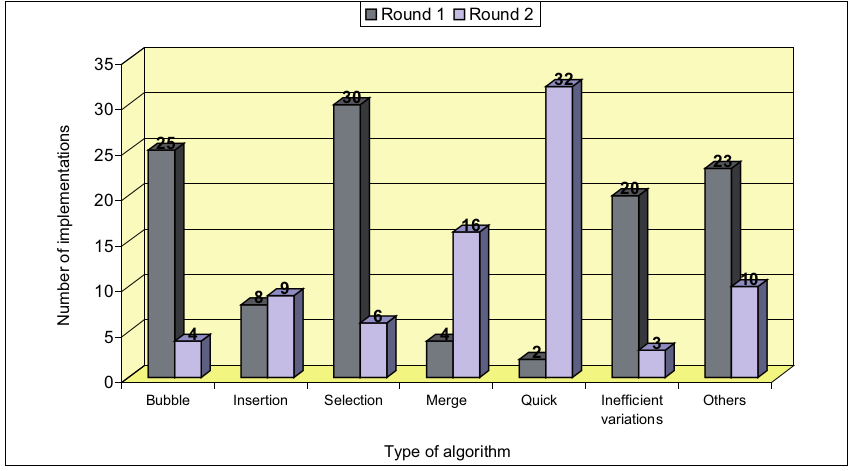
\includegraphics[scale=0.4]{imagem/clusterManual.png}
	        \captionsetup{justification=centering}
	        \caption{Agrupamento manual das implementações dos estudos estudantes na
	        primeira e segunda etapa \cite{Taherkhani:2012}.}
	        \label{fig:clusterManual}
	    \end{figure}
	    
	    Após o agrupamento manual dos métodos de ordenação implementados pelos alunos,
	    \citeonline{Taherkhani:2012} realizou o reconhecimento automático das
	    implementações por meio da ferramenta Aari. Inicialmente a ferramenta foi
	    treinada para reconhecer os algoritmos de ordenação citados anteriormente.
	    A \cref{fig:clusterAutomatico} apresenta um gráfico para comparar cada
	    agrupamento manual realizado anteriormente com o reconhecimento automático
	    da ferramenta. Possui as mesmas propriedades da \cref{fig:clusterManual}
	    com exceção das colunas. A coluna da esquerda referencia o agrupamento manual
	    de cada algoritmo de ordenação da segunda etapa e a coluna da direita apresenta
	    os algoritmos reconhecidos corretamente pelo Aari. Nota-se que todas as
	    implementações dos métodos de ordenação \foreign{bubble sort},
	    \foreign{selection sort} e \foreign{quicksort} foram classificados corretamente.
	    É possível verificar também que a ferramenta não foi capaz de reconhecer vários
	    algoritmos como \foreign{others}, visto que ele não foi treinado para
	    reconhecer tais algoritmos.
	    
	    \begin{figure}[ht]
	        \centering
	        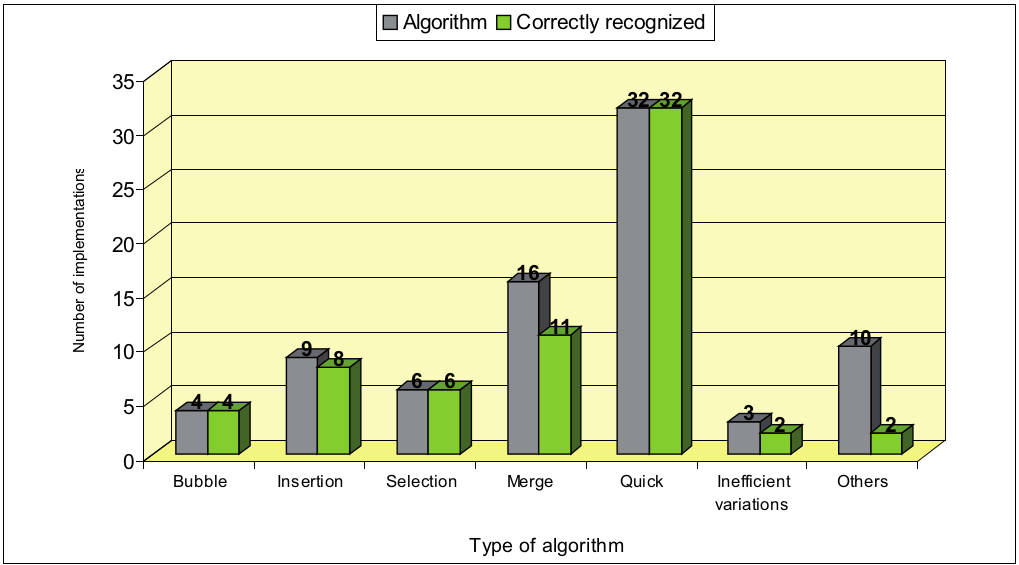
\includegraphics[scale=0.33]{imagem/clusterAutomatico.png}
	        \captionsetup{justification=centering}
	        \caption{Comparação das implementações dos alunos dos \foreign{clusters}
	        manual e automático da segunda etapa \cite{Taherkhani:2012}.}
	        \label{fig:clusterAutomatico}
	    \end{figure}
	    
	    A ferramenta mostrou-se capaz de identificar a maioria dos métodos de ordenação
	    para quais foi treinada previamente. Tal abordagem torna-se interessante quando
	    há um plano de ensino detalhando os problemas a serem resolvidos, possibilitando
	    o treinamento da ferramenta. Entretanto, caso seja utilizado para classificar
	    diversos problemas desconhecidos para o classificador, não há uma categorização
	    prévia adequada. Desta forma, inviabilizaria sua utilização em MOOCs se fosse
	    utilizado para classificar os problemas de todos os cursos de programação.
	    
	    \citeonline{Glassman:2015} apresentam o OverCode, ferramenta de visualização
	    de informação que mostra os \foreign{clusters} formados, as principais
	    instruções utilizadas pelas implementações presentes em um determinado
	    agrupamento e as linhas de código de uma determinada função/método. A
	    ferramenta é voltada para aqueles que realizarão a correção das submissões.
	    
	    Para verificar a similaridade das submissões a fim de realizar o agrupamento,
	    é necessário: formatar o código-fonte, executar um caso de teste, extrair a sequência
	    de variáveis, identificar variáveis em comum, renomear variáveis comuns e únicas
	    para, então, realizar o agrupamento. Formatar o código-fonte consiste na refatoração
	    em cada implementação. Essa refatoração consiste na remoção dos espaços entre os
	    \foreign{tokens}, mantendo os espaços somente após as palavras reservadas, de
	    comentários e de linhas em branco. Essas modificação no código-fonte, além de
	    deixá-lo legível, também permite cada linha de código ser representada como
	    uma \foreign{string} para que seja possível encontrá-lo em outras soluções.
	    
	    A segunda etapa do agrupamento consiste na execução do mesmo caso de teste
	    para todas as implementações. A cada passo da execução, os nomes e valores de
	    variáveis locais e globais, bem como o valor de retorno da função são gravados
	    como se fosse um histórico de execução ou \foreign{trace}. A partir desse
	    histórico, a ferramenta extrai a sequência de valores de todas as variáveis.
	    
	    A partir do conhecimento da sequência de valores de cada variável, o OverCode
	    identifica quais são as variáveis comuns. Tais variáveis são reconhecidas a
	    partir das suas sequências idênticas dado dois ou mais históricos de execução.
	    As variáveis que só ocorrem uma vez no \foreign{trace} são as variáveis únicas.
	    Após reconhecer as variáveis comuns e únicas, a ferramenta renomeia-as para o
	    nome da variável que ocorreu em mais históricos de execução. Após todos esses
	    passos, o agrupamento é realizado por meio de comparação de blocos de código
	    idênticos.
	    
	    \begin{figure}[ht]
	        \centering
	        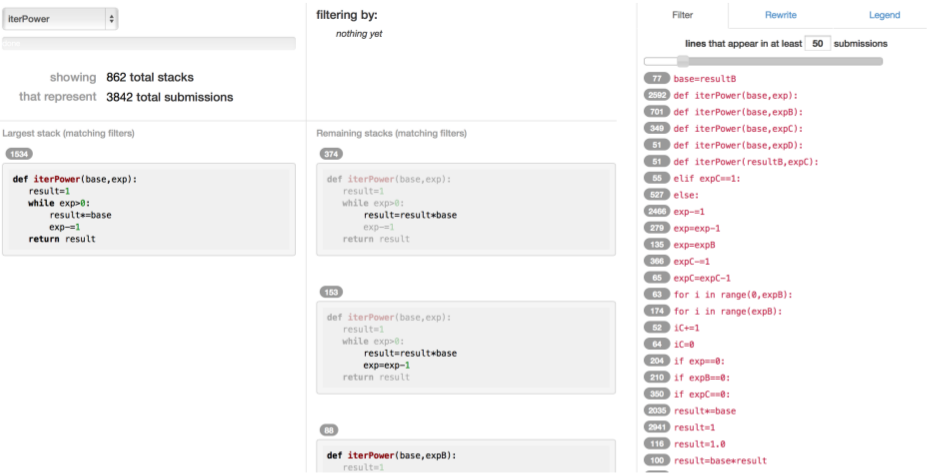
\includegraphics[scale=0.4]{imagem/overCode.png}
	        \captionsetup{justification=centering}
	        \caption{Interface da ferramenta OverCode \cite{Glassman:2015}.}
	        \label{fig:interfaceOverCode}
	    \end{figure}
	    
		Na \cref{fig:interfaceOverCode} é possível notar a utilização das pilhas
		(\foreign{stacks}) para representar os agrupamentos. A primeira coluna da
		esquerda exibe dois painéis. O primeiro painel apresenta o número de
		agrupamentos, representado pelas pilhas, e o número total de submissões,
		enquanto o segundo painel, mostra a maior \foreign{stack}. A coluna central
		apresenta a opção de busca, filtrando por uma determinada palavra no quadro
		superior, e as pilhas remanescentes no quadro inferior. Enquanto a terceira
		coluna apresenta a frequência com que as linhas de códigos estão presentes
		nas soluções das pilhas.

		A comparação das pilhas menores com a pilha maior ocorre entre a primeira e a
	    segunda coluna dando ênfase nas linhas que estão implementadas diferentes. Com
	    isso, é possível verificar como cada pilha foi montada e a característica daquela
	    pilha quando comparada com a pilha maior. Como utiliza análise dinâmica, extraindo
	    o histórico de execução para agrupar as submissões, é possível verificar o \foreign{trace}
	    de uma variável ao longo de sua execução em um caso de teste a fim de auxiliar os
	    usuários a entenderem a execução do algoritmo.
	    
		\begin{figure}[h]
			\centering
			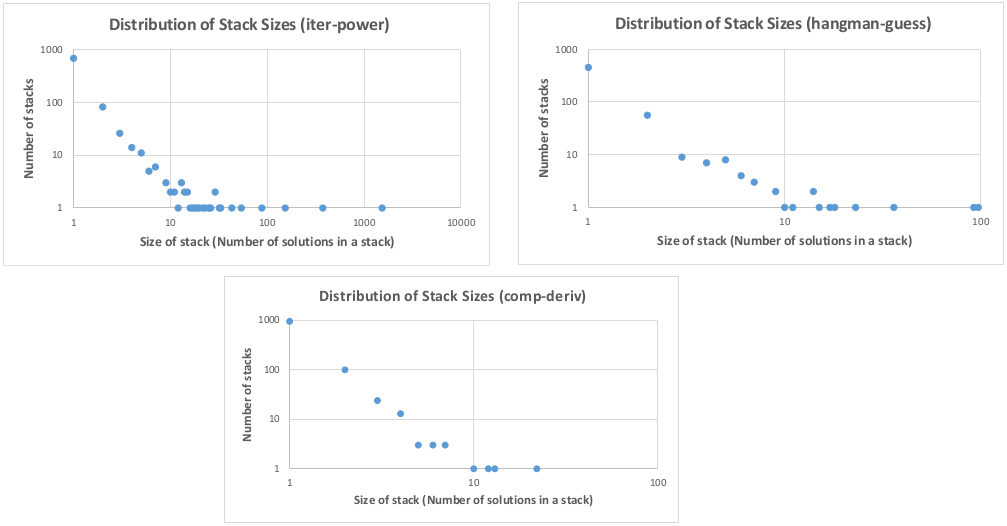
\includegraphics[width=1\linewidth]{imagem/OverCodeDistri}
			\caption{Representação do tamanho dos agrupamentos (pilhas) para cada problema
				\cite{Glassman:2015}}
			\label{fig:OverCodeDistri}
		\end{figure}

		A \cref{fig:OverCodeDistri} apresenta o agrupamento, representado pela quantidade de
		pilhas no eixo $y$ e o total de submissões em uma pilha no eixo $x$,  em relação a
		três problemas resolvidos em Python: o problema \texttt{iterPower} refere-se a
		implementação de uma função, que possui a base e o expoente como parâmetros, para
		calcular o exponencial com sucessivas multiplicações; o problema \texttt{hangman}
		possui um vetor de caracteres (\foreign{string}) e uma lista de caractere como
		parâmetros, na qual deve retornas todos os caracteres da \foreign{string} que não
		estão presentes na lista de caracteres; por fim, o problema \texttt{compDeriv}
		calcula a derivada de um polinomial, no qual os coeficientes estão presentes em
		uma lista. Esses problemas obtiveram 3875, 1118 e 1433 soluções corretas submetidas,
		respectivamente. Na devida ordem, a maior pilha de cada problema são constituídas
		de 1534, 97 e 22 implementações e 684, 452 e 959 pilhas com apenas uma solução.

	    Por fim, os autores concluíram que a interface auxilia os professores a terem
	    uma visão de alto nível das soluções (implementações). Podendo compreender os
	    erros e fornecer um \foreign{feedback} mais relevante, devido ao agrupamento
	    das implementações. O que diminui consideravelmente a quantidade de submissões
	    a serem efetivamente corrigidas.
	    
		A análise dinâmica e os recursos realizados para que fosse montado a pilha
		mostrou-se eficiente, principalmente para o problema \texttt{iterPower}, no
		qual sua maior pilha obteve quase 40\% das implementações corretas. Com isso,
		torna-se evidente o quanto a ferramenta pode auxiliar os professores a realizar
		as correções dos códigos-fontes. A etapa de padronização do código realizado
		durante a análise \foreign{pipeline}, no qual verifica-se as variáveis comuns
		e renomeia-as, contribui com a comparação bloco a bloco, devido a partes do bloco,
		onde ocorrem a utilização dessas variáveis, serem parecidas. Poderia ter sido
		verificado todos os problemas implementados em apenas um código-fonte para
		verificar qual seria o resultado dos agrupamentos e compará-los.
	    
	    \citeonline{Wei2015} apresentam uma ferramenta para auxiliar na correção das
	    submissões dos MOOC's de forma a agrupar pedaços (\foreign{chuncks}) de códigos
	    fontes semelhantes, agrupá-los conforme sua similaridade e alocar cada conjunto
	    de implementações ao estudante com conhecimento suficiente para revisá-los.
	    
	    Foi necessário realizar o particionamento do código para torná-lo legível
	    e fácil de compreender. Os pedaços foram extraídos das implementações como
	    se fossem funções. Entretanto, há uma dificuldade para verificar as submissões
	    quando ocorria uma chamada de função em uma outra função, dificultando a divisão
	    em pedaços do código. Também foi necessário normalizar cada submissão a fim de
	    encontrar o estilo de escrita, visto que até mesmo o nome da variável pode
	    alterar o estilo de escrita.
	    
	    A ferramenta desenvolvida por \citeonline{Wei2015} normaliza o código por
	    meio de três regras:
	    
	    \begin{enumerate}
	    	\item Remoção de espaços, linhas em branco e comentários;
	    	\item Exclusão de palavras reservadas da linguagem de programação,
	    	identificadores predefinidos e nomes de funções de bibliotecas;
	    	\item E substituição dos identificadores de variáveis do usuário por um
	    	símbolo especial.
	    \end{enumerate}
	    
	    Com isso foi calculado um valor \foreign{hash},representando cada \foreign{substring}
	    de um código-fonte, a fim de verificar a similaridade do estilo de escrita \foreign{token}
	    a \foreign{token} e utilizado o algoritmo de \texttt{winnowing} \cite{schleimer2003}
	    para escolher o menor subconjunto do estilo de escrita a fim de realizar as
	    comparações por meio do coeficiente de similaridade de \foreign{Jaccard} \cite{jaccard1901}. E
	    com a finalidade de identificar a dificuldade da implementação, foi utilizado
	    a distância Euclidiana para comparar as características extraídas -- quantidade
	    de métodos invocados e laços de repetição aninhados -- e o \foreign{K Nearest Neighbor}
	    (\texttt{k-NN}) para identificar o nível de dificuldade de revisão do
	    \foreign{chunck}.
	    
		\begin{figure}
			\centering
			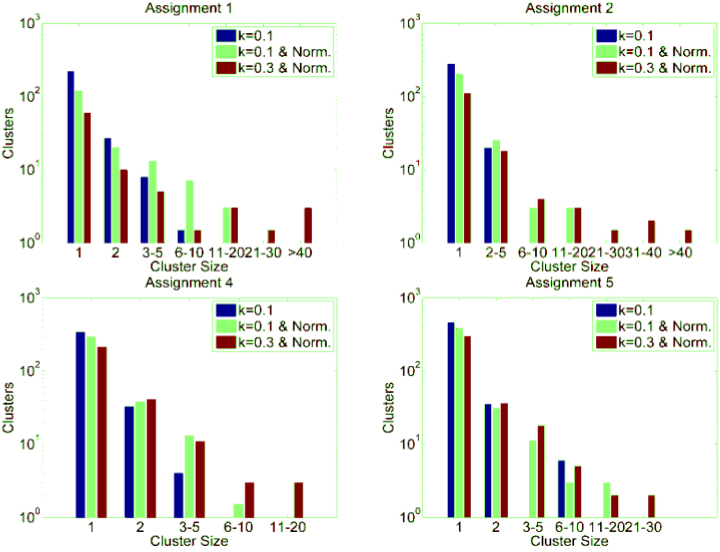
\includegraphics[width=0.7\linewidth]{imagem/clusteringPerformance}
			\captionsetup{justification=centering}
			\caption{Distribuição dos agrupamentos \cite{Wei2015}.}
			\label{fig:clusteringPerformance}
		\end{figure}
	    
		A \cref{fig:clusteringPerformance} apresenta a distribuição dos
		agrupamentos em quatro problemas distintos. Para todos os gráficos, a
		abcissa é referente ao tamanho dos pedaços, enquanto a ordenada representa
		o número de agrupamentos. É possível notar três tipos de agrupamento. A barra
		horizontal azul representa o agrupamento sem normalização. enquanto as barras
		verde e vermelho possuem o valor de $k$ diferente, entretanto, ambas estão
		normalizadas. Há uma diferença entre as tarefas 1 e 2 e, as tarefas 4 e 5:
		os dois primeiros só possuem apenas uma função para resolver um pequeno problema,
		Contudo, as demais tarefas possuem implementações com várias funções. Enquanto
		as tarefas 1 e 2 apresentaram bons agrupamentos e o tamanho dos grupos era
		condizente com a quantidade de estudantes (200) quando $k$ era igual a 3.0.
		As tarefas 4 e 5 não foram satisfeitas devido ao total de pedaços em um grupo
		ser próximo de 20 e o restante dos códigos formaram pequenos agrupamentos.
		
		Conforme a \cref{fig:clusteringPerformance}, pode-se notar que a
		distribuição dos \foreign{chuncks} sem normalização de código é inadequado,
		visto que vários pedaços em todas as tarefas estavam sozinhos, e o maior
		agrupamento possuía entre 6 a 10 funções. Enquanto a tarefa 1 e 2 apresentou
		bons agrupamentos, nos quais possuíam mais de 40 implementações em um mesmo
		grupo quando $k$ era igual a 3.0. As tarefas 4 e 5 não foram satisfeitas devido
		a cada código-fonte conter várias funções, principalmente quando não normalizados.
		
		É possível notar que a abordagem dos códigos-fontes compostas de diversas
		funções (tarefas 4 e 5) não obteve sucesso, pois, independente da tarefa
		selecionada, nota-se que a maioria dos \foreign{clusters} formados possuíam
		apenas um código-fonte. Entretanto, a submissão de implementações contendo
		apenas uma função (tarefas 1 e 2) para resolver o problema torna-se interessante,
		devido a realização de alguns agrupamentos com mais de 40 implementações
		semelhantes. Em um ambiente controlado, no qual todos os alunos irão submeter
		diversas soluções com somente uma função, é interessante a utilização da
		ferramenta. Caso contrário, seu uso não interferirá significativamente no
		auxilio a correções de códigos-fontes. 
		
		\begin{landscape}
			\begin{table}[h]
				\tiny
				\begin{tabularx}{\linewidth}{ |X|X|X|X|X|X|X| }
					\hline % Primeira linha
					Artigos
					& Dados de entrada
					& Característica extraídas dos dados de entrada
					& Algoritmo para cálculo de distância ou similaridade
					& Algoritmo de clusterização / Classificador
					& Avaliação
					& Conclusões \\
					\hline % Segunda Linha
					\citeonline{Yin:2015}
					& Implementações
					& Árvore de sintaxe abstrata
					& Distância de Edição de TED normalizada que utiliza estrutura
					\foreign{top-down} e pontuação silhueta
					& DBSCAN e OPTICS
					& Clusterização de algoritmos baseado nas soluções de um problema.
					Em cada \foreign{cluster}, identifica as diferenças nas
					implementações de uma abordagem particular
					& TED normalizado demonstra conjuntos mais estáveis e menos discrepantes \\
					\hline % Terceira linha
					\citeonline{Glassman:2014}
					& Implementações
					& Linguagem de alto nível: 12 características - posição de declarações
					condicionais em relação a instruções de \foreign{loop}, profundidade
					dos \foreign{loops} aninhados, números de nós AST, instruções de
					retorno, laços, comparações, etc. Linguagem de baixo nível: 48
					características - operações aritméticas, comparações, \foreign{loops},
					funções de bibliotecas, declarações, número de variáveis do programa,
					valores constantes, etc.
					& Informação Mútua Ajustada
					& K-means
					& Utilizando a métrica AMI comparando os \foreign{cluters} dos feitos
					pelos professores, no qual 0 indica agrupamentos puramente independentes
					e 1, perfeita concordância entre os agrupamentos.
					& Para k maior ou igual a 15, encontrou-se alta concordância entre os
					\foreign{cluster} do k-means e do professor \\
					\hline % Quarta linha
					\citeonline{Taherkhani:2012}
					& Implementações
					& Características numéricas: NAS, LoC, MCC, N1, N2, n1, n2, N, n, Nov,
					NoL, NoNL, NoB. Características descritivas: recursivo, \foreign{tail
					recursive}, funções de variáveis, \foreign{array} auxiliar. Outras
					características: informações de \foreign{loop}/bloco, informações do
					contador de laço, informações de dependência. Características de algoritmos
					de ordenação: MWH, TEMP, In-place, OIID e IITO.
					& Vetor de características,calculada a partir das características extraídas
					das implementações
					& C4.5 (árvore de decisão)
					& Com os algoritmos da primeira rodada, obteve 71\% de precisão; da
					segunda rodada, 81\%.
					& Bom reconhecimento do algoritmo, se estiver conforme a teoria. Taxa de
					acerto considerável baseado em um possível erro do professor. Utilização
					semiautomática: o Aari corrige partes do trabalho no qual foi treinado e
					o professor, o restante \\
					\hline % Quinta linha
					\citeonline{Glassman:2015}
					& Implementações
					& Rastro do programa (Sequência de variáveis, variáveis comuns e
					renomeação de variáveis: colisão comum / comum; colisão de múltiplas
					instâncias; e colisão único/comum), blocos de código.
					& Análise \foreign{pipeline}
					& Comparação entre conjuntos de linhas de código
					& Grande quantidade de pilhas com poucos blocos de código-fonte e poucas
					pilhas com grande quantidade de blocos implementados
					& A partir do OverCode e as pilhas com os algoritmos divididos pelas
					características extraídas, dá a possibilidade de retornar um
					\foreign{feedback} mais preciso para cada grupo e facilita a observação
					da solução do problema. \\
					\hline % Sexta linha
					\citeonline{Wei2015}
					& Implementações
					& Normaliza o código e considera apenas o estilo de escrita do estudante
					& Coeficiente de similaridade de Jaccard
					& Algoritmo \foreign{Winnowing}
					& Classificação de \foreign{workload}: distância Euclidiana e k-NN
					& A agrupamento por pedaços de código aumentou sua eficiência. \\
					\hline
				\end{tabularx}
				\captionsetup{justification=centering}
				\caption{Principais informações dos trabalhos relacionados}
				\label{tab:caracPrinc}
			\end{table}
		\end{landscape}
		
		A \cref{tab:caracPrinc} apresenta as principais características de cada trabalho
		relacionado importantes para o desenvolvimento desse projeto. Possibilitando a
		comparação dos tipos de análises utilizados, quais características foram
		extraídas a partir dessas análises e qual abordagem obteve melhor desempenho. 
\chapter{Métodos e ferramentas}
\label{chap:metodos-ferramentas}

	Neste capítulo será apresentado o método utilizado, os resultados obtidos durante
	o desenvolvimento deste estudo conforme a \cref{fig:fluxogramaProposta},o qual
	apresenta as fases: definição da linguagem de programação e das características
	a serem extraídas; códigos-fontes; extração de características; mineração de dados e
	agrupamento; e projeção e visualização. A linguagem de programação escolhida foi \texttt{Python},
	as características serão originadas pela análise estática e do estilo de escrita,
	os códigos-fontes consiste em duas base de dados distintas, a extração
	de características ocorreu por meio de ferramentas disponibilizadas livremente, a
	mineração e agrupamento dos dados foi realizada utilizando a similaridade do
	cosseno, enquanto a projeção e a visualização dos dados foi realizada pela ferramenta
	\texttt{Science View}.
	 % TODO: mencionar que este capítulo é uma instância do método apresentado no capítulo anterior, considerando as fases XYZ. Explique em uma linha o que foi feito para cada fase.
	 


 	\section{Método}
	 	Após a revisão da literatura, verificamos que o projeto é baseado em algumas etapas.
	 	Conforme a \cref{fig:fluxogramaProposta}, é necessário escolher qual linguagem de programação
	 	será utilizado. Em seguida deve-se verificar quais características podem ser extraídas
	 	das implementações submetidas utilizando a linguagem especificada. Posteriormente, é
	 	necessário construir a base de dados por meio da submissão de implementações, realizar
	 	a extração de características, minerar os dados extraídos das submissões e verificar a
	 	similaridade entre as implementações. Por fim, realizar a projeção e visualizar os
	 	agrupamentos.
	 	
	 	\begin{figure}[h]
	 		\centering
	 		\includegraphics[width=0.7\linewidth]{imagem/fluxogramaProposta}
	 		\caption{Fluxograma das etapas necessárias para a realização do projeto}
	 		\label{fig:fluxogramaProposta}
	 	\end{figure}
	 	
	 	A \textbf{linguagem de programação} refere-se a definição de qual linguagem será
	 	utilizada para o desenvolvimento do projeto. Por exemplo: \texttt{C}, \texttt{Java}
	 	ou \texttt{Python}. Deve ser escolhida conforme a demanda da sua utilização, pela
	 	disponibilidade de cursos de programação ofertado em \acs{MOOC}s ou pelo conhecimento de
	 	ferramentas que possam verificar características dessa linguagem, como o
	 	\texttt{cpplint} para a linguagem \texttt{C}, \texttt{Checkstyle} para
	 	\texttt{Java} e \texttt{PEP8} para \texttt{Python}.
	 	
	 	A etapa seguinte \textbf{definir características a serem extraídas} será realizado
	 	com base nos trabalhos relacionados (\cref{sec:TrabRel}). Verificamos que é
	 	possível utilizar características originadas de um tipo de análise (estática,
	 	dinâmica e do estilo de escrita), bem como associar características de análises
	 	distintas para obter um melhor resultado.
	 	
	 	O estágio \textbf{códigos-fontes} refere-se à construção da base de dados que será
	 	utilizada no experimento. Tal base tem que possuir uma quantidade considerável de
	 	submissões de códigos-fontes, devido a quantidade de usuários que utilizam o \acs{MOOC},
	 	para que seja possível avaliar o desenvolvimento do projeto com uma quantidade
	 	condizente com o número de usuários.
	 	
	 	A \textbf{extração de características} é a fase na qual escolhe-se uma ferramenta
	 	disponibilizada livremente pela Internet que forneça os dados necessários, visto
	 	que não desejamos criar uma ferramenta para esse fim. Tal estágio é responsável pela
	 	adaptação das ferramentas selecionadas anteriormente para que seja possível obter
	 	as características e salvá-la em algum tipo de arquivo, como o formato \texttt{XML}
	 	e o \texttt{CSV}, por exemplo.
	 	
	 	Na etapa \textbf{mineração de dados e agrupamento} analisa-se os dados obtidos a
	 	fim de verificar um padrão das características obtidas. Isso permite a utilização
	 	de técnicas para verificar a similaridade dos códigos-fontes a fim
	 	de produzir os agrupamentos.
	 	
	 	Por fim, \textbf{projeção e visualização} refere-se ao emprego de técnicas de
	 	projeção para que seja possível diminuir a quantidade de dimensões. Uma dimensão
	 	é referente a uma característica extraída da implementação, portanto a quantidade
	 	de dimensões é igual a quantidade de características extraídas. Com isso, é
	 	necessário selecionar uma técnica para diminuir um espaço n-dimensional para
	 	duas ou três dimensões a fim de realizar a visualização dos agrupamentos.
	 	
	 	No caso das características extraídas não forem relevantes para a formação de
	 	agrupamentos ou a visualização não produzir modelos gráficos significativos por
	 	meio dos mapeamento de dados realizados pela técnica de projeção, será necessário
	 	voltar a segunda etapa para definir outras características a serem extraídas.
	 	
	 	Nosso objetivo, por meio dessas etapas, consiste no desenvolvimento de subsídios
	 	de avaliação, utilizando técnicas de visualização para auxiliar os professores a
	 	corrigirem todas as submissões, considerando o tempo e a qualidade do \foreign{feedback},
	 	principalmente. Por isso, teremos três questões de pesquisa (QP):
	 	
	 	\begin{itemize}
	 		\item \textbf{QP$_1$}: o algoritmo de agrupamento produz grupos de códigos-fontes
	 		com boa qualidade?
	 		\item \textbf{QP$_2$}: a utilização de subsídios de avaliação reduz o tempo % TODO: retirar tempo e abordar isso nas conclusões como trabalhos futuros
	 		de correção de todas as submissões?
	 	\end{itemize}
	 	
	 	O subsídio de avaliação será uma adaptação da \texttt{Science View} \cite{Alencar-etal:2012}
	 	que, originalmente, verifica as mudanças nas relações de documentos com o decorrer do tempo,
	 	utilizando técnicas de mineração, projeção e visualização. Com isso, teremos as
	 	seguintes hipóteses (HP) em relação a utilização da proposta deste estudo:
	 	
	 	\begin{itemize}
	 		\item \textbf{HP$_1$}: tempo para corrigir os exercícios com os subsídios é inferior  % TODO: mudar esta hipótese para avaliar a qualidade da visualização
	 		ao tempo necessário com a correção manual;
	 	\end{itemize}
	 	
	 	Para validar o tempo gasto e a qualidade dos \texttt{feedbacks} para todas as correções,
	 	será criado dois grupos de professores. Um grupo utilizou a técnica proposta nessa pesquisa para
	 	realizar a avaliação das implementações, enquanto o outro grupo avaliou as submissões
	 	manualmente. Além disso, a qualidade dos \foreign{feedbacks}, será avaliado através de \foreign{survey}
	 	e questionário para cada aluno sobre o \foreign{feedback} que recebeu e também será avaliado
	 	por meio de submissões futuras, visto que a ferramenta realiza várias projeções ao longo do tempo.

	
	\section{Considerações para avaliações}

		% TODO: inserir um texto nesta linha: Considerando os estágios estabelecidos no método
		% descrito na seção anterior, foram definidos requisitos e elementos a serem empregados
		% na avaliação de programas [...]

		\subsection{Definição da linguagem de programação}
			Foi definido a utilização da linguagem de programação Python. A escolha foi
			devido ao conhecimento prévio de ferramentas que possam auxiliar na verificação
			e extração de características, bem como a disponibilidade de cursos sobre
			introdução a programação, utilizando \texttt{Python}, em diversos \acs{MOOC}s.

		\subsection{Definição das características a serem extraídas}
			Considerando a combinação de características originadas de tipos de análises
			distintas, utilizamos uma combinação de aspectos provenientes da análise  % TODO: a banca apresentou dúvidas o que seriam tais características. Isso é sinal de que precisamos melhor a descrição do capítulo 2. Além disso, parte das informações apresentads na seção "Extração de características" deve vir pra cá (não é necessário colocar partes sobre ferramenta utilizada, mas precisamos informar que foram selecionadas as características de quantidades de linhas de código, complexidade ciclomática e quantidade de violações de regras de estilo de escrita definida pelo PEP8).
			estática e do estilo de escrita. A escolha da análise estática se dá pela
			possibilidade de implementações para solucionar o mesmo problema possuírem
			o mesmo tamanho. Enquanto a organização do código, realizado pelo programador,
			pode impactar no entendimento da solução do problema, por isso a escolha da
			análise do estilo de escrita. Para isso, utilizaremos a ferramenta \texttt{Flake8}
			\cite{flake8} que pode adquirir todas as características necessárias por meio da
			utilização de \foreign{plugins}. Não utilizaremos a análise dinâmica pela falta
			de conhecimento de ferramentas que nos forneça tal característica e pelo pouco
			tempo hábil para implementação de uma ferramenta para realizar esse tipo de
			análise e validação dessa ferramenta.
			
			As características a serem extraídas da análise estática serão apenas a quantidade
			de linhas de código e a complexidade ciclomática da implementação. Em relação
			a análise do estilo de escrita, será considerado todas as violações do estilo de
			escrita definido pelo \texttt{PEP8} \cite{van2001pep}. 

		\subsection{Códigos-fontes}	
			Essa etapa refere-se a construção da base de dados que será utilizada no experimento.
			É necessário que o conjunto de implementações obtenha uma quantidade considerável de
			códigos-fontes a fim de avaliar a utilização da ferramenta para \acs{MOOC}. A
			base de dados desse estudo possui somente implementações desenvolvidas em \texttt{Python}.
			
		\subsection{Extração de características} % TODO: citar que foram escolhidas características por conveniência, mas que isso não afeta a qualidade das projeções com relação aos critérios escolhidos (desde que posteriormente sejam escolhidas características mais interessantes para a avaliação -> trabalho futuro)		
			Obtivemos as informações necessárias por meio da análise estática e do estilo de   
			escrita com o auxílio das ferramentas \texttt{PEP8} \cite{pep8} e \texttt{McCabe}
			\cite{mccabe} que funcionam como \foreign{plugins} para o \texttt{Flake8}.
			Extraímos da análise estática, além do estilo de escrita, a quantidade de linhas do código-fonte e a complexidade ciclomática de cada \foreign{plugin}, respectivamente. Contudo, o
			foco do \texttt{PEP8} é verificar se o estilo de escrita PEP 8 \cite{van2001pep}
			está sendo praticado corretamente. Por esse motivo, extraímos as características
			relacionadas a: indentação (\cref{tab:pep8E100}); espaços em branco
			(\cref{tab:pep8E200}); linhas em branco (\cref{tab:pep8E300}); declaração de
			importação de bibliotecas (\cref{tab:pep8E400}); tamanho da linha (\cref{tab:pep8E500});
			quantidade de instruções por linha e formas de instrução (\cref{tab:pep8E700}); por fim,
			verificação de sintaxe e geração de \foreign{tokens} (\cref{tab:pep8E900}).
		
%	A indentação possui as seguintes características: tabulações e espaços misturados;
%	o nível não possui indentação, mas foi encontrado espaços em branco ou uma indentação,
%	ambas podendo ser seguida de um comentário; o nível possui uma indentação, entretanto,
%	esse não foi encontrado ou foi encontrado seguido de um comentário; há espaços, contudo
%	é menor que uma tabulação de 4 espaços, definido como padrão no \texttt{PEP8}; e em
%	instruções de múltiplas linhas verifica se as linhas seguintes estão indentadas com
%	a primeira linha da instrução.
%	
%	Os espaços em branco são analisados em chamadas de função, atribuições, operações
%	lógicas e aritméticas, entre palavras reservadas e comentário. Em chamadas de
%	funções constata a presença ou falta de espaço em branco depois dos \foreign{tokens}
%	\texttt{(}, \texttt{\{} e \texttt{[} ou antes dos \foreign{tokens} \texttt{)},
%	\texttt{\}}, \texttt{]}, como também antes de \texttt{(} e \texttt{[} no caso de
%	querer acessar um índice de uma lista, por exemplo. Nas atribuições compreende se
%	não há espaço em branco entre o operador de atribuição, enquanto nas operações
%	lógicas e aritméticas constata se não há espaço entre seus operadores.
%	
%	% linhas em branco entre métodos e, entre declaração da classe e um método da classe
%	A verificação de linhas em brancos é utilizada para observar como um método está
%	separado de outro método, bem como da declaração da classe. Os métodos devem estar
%	separados por duas linhas em branco, enquanto a declaração da classe e o primeiro
%	método deve estar separado por apenas uma linha em branco. Caso essas duas
%	características não sejam cumpridas, além de possuir várias linhas em branco,
%	o analisador gera um erro.
%	
%	% importação de bibliotecas
%	A quantidade de bibliotecas que estão sendo importadas também é observado. O
%	\texttt{PEP8} considera importar apenas uma biblioteca por linha. Portanto,
%	o \foreign{plugin}, irá detectar a importação de duas ou mais bibliotecas na
%	mesma linha.
%	
%	% tamanho da linha
%	O analisador também verifica o tamanho, em caracteres, de uma linha. Uma mensagem
%	de erro ocorre quando a linha possuir 80 caracteres ou mais. Além disso, é
%	contraindicado utilizar uma barra invertida seguido de uma nova linha quando estiver
%	entre colchetes ou parenteses.
%	
%	% quantidade de instruções por linha e formas de instrução
%	A quantidade de instruções por linha menciona as instruções que podem ser separadas
%	por \texttt{:} (dois-pontos) ou \texttt{;} (ponto e vírgula). O primeiro caso pode
%	ocorrer em uma declaração de condicional e sua primeira instrução. Enquanto, o segundo
%	caso, ocorre entre duas instruções. Por fim, as formas de instruções verifica: se uma
%	instrução é terminada com \texttt{;}; utilização de operadores lógicos para comparar
%	valores únicos (\foreign{singletons}), ao invés de utilizar \texttt{is} ou \texttt{is not};
%	a utilização de \texttt{not in} para verificar se uma variável está contida em outra e
%	\texttt{is not} para comparar objetos; por fim, a comparação de tipos é realizado pelo
%	\texttt{isinstance()}.
%	
%	% verificação de sintaxe e geração de tokens
%	Por fim, o \texttt{PEP8} também verifica se a sintaxe do código-fonte é valida.
%	\textbf{Falta falar sobre o erro E902, mas não entendi a definição no PEP8:
%		"Tokenize the file, run physical line checks and yield tokens."}
	
			A ferramenta \texttt{mccabe} \cite{mccabe2013} fornece informações sobre a
			complexidade ciclomática \cite{mccabe} de cada função ou método implementado.
			Essa complexidade é referente às estruturas de decisões implementadas \cite{mccabe},
			ou seja, seu cálculo é realizado com base na utilização de \texttt{if/else} e laços
			de repetição.
			
		
		\subsection{Mineração de dados e agrupamento}
			Com a finalidade de encontrar relações entre as características extraídas, em
			conformidade com a etapa Extração de Padrões (\cref{fig:mineracaoDados}).
			Utilizamos a técnica de similaridade do cosseno. Sua escolha ocorreu pelo fato de obtermos
			uma matriz esparsa -- possui grande quantidade de 0 (zeros) -- ao realizar o
			Pré-Processamento (\cref{fig:mineracaoDados}) das características extraídas. A
			ocorrência da grande quantidade de 0 (zeros) ocorre pela busca dos programadores
			em implementar suas soluções computacionais corretamente. Além disso, faz com que
			implementações para problemas distintos não sejam consideram semelhantes devido a
			quantidade de 0 (zeros) nas mesmas características. A grande quantidade de 0 (zeros)
			pode ser observada na \cref{fig:arquivoCSV}.
		
		\subsection{Projeção e visualização}
			Para possibilitar a visualização dos agrupamentos utilizaremos a \texttt{Science View}
			\cite{Alencar-etal:2012} que utiliza o algoritmo de agrupamento \acs{DBSCAN} \cite{Ester1996}
			e a técnica de projeção multidimensional dinâmica \ac{T-LSP} \cite{Alencar}. Até o momento,
			realizamos a adaptação para leitura do arquivo no formato \texttt{CSV}. A \acs{T-LSP} \cite{Alencar}
			produz uma sequência temporal de mapas conforme a similaridade dos dados. Com isso, poderemos
			verificar se o aluno está progredindo no curso, visto que a técnica de projeção permitirá
			visualizar projeções relativas a implementações por semana ou meses, por exemplo. Desta
			forma, poderemos obter sequências temporais de mapas baseado na similaridade das
			implementações de um único aluno.
			
			% TODO: Marco: escrever sobre como a projeção pode ser utilizada para avaliação de trabalhos: requisitos
			% e instruções com a ScienceView
			
				
		
		
	\section{Ferramentas}


		\subsection{ScienceView-Python}
		\label{sec:scienceView-Python}
			% TODO: descrever

			% TODO: melhorar este início (ele estava em outra parte do texto). Acrescente uma frase sobre a importância de extrair as características e disponibilizá-las em um formato adequado para a ferramenta de visualização (justificando assim as modificações relatadas a seguir)
			Para extrair as características das implementações, foi necessário a modificação
			das ferramentas \texttt{PEP8} e \texttt{Flake8}. No \texttt{PEP8}, alteramos o
			método \texttt{check\_files()} que é chamado apenas uma vez e é responsável por
			verificar cada código-fonte especificado no momento da execução por linha de
			comando. Tal modificação consiste na criação do arquivo no formato \texttt{CSV}
			com o cabeçalho: nome do arquivo, total de linhas do código-fonte, quantidade
			de erros do estilo de escrita e cada erro do \texttt{PEP8}.
			
			\begin{figure}[h]
				\centering
				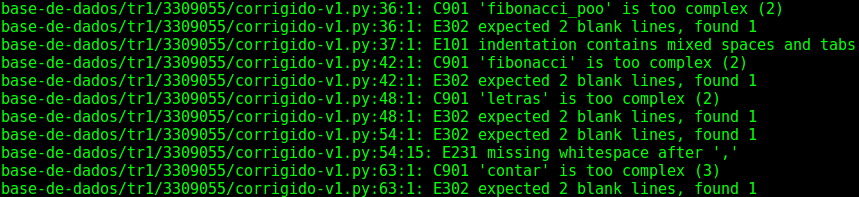
\includegraphics[width=1\linewidth]{imagem/flake8}
				\caption{Representação das características analisadas pelo \texttt{Flake8}}
				\label{fig:flake8}
			\end{figure}
			
			A \cref{fig:flake8} apresenta o formato da impressão de cada característica do
			\texttt{Flake8}. Notamos que era possível obter as características no momento em
			que fosse realizado cada \texttt{print} dos dados, visto que, todas as linhas
			possuem o tipo do erro, E302 ou a complexidade ciclomática C901, por exemplo.
			Desta forma, alteramos o método \texttt{get\_file\_result()} da classe
			\texttt{reporter} do \texttt{Flake8}. Criamos um dicionário contendo todos os
			erros do \texttt{PEP8} e do \texttt{mccabe} como chave. A cada impressão
			verificamos qual é o tipo do erro e incrementamos o valor dessa chave.
			
			\begin{figure}[h]
				\centering
				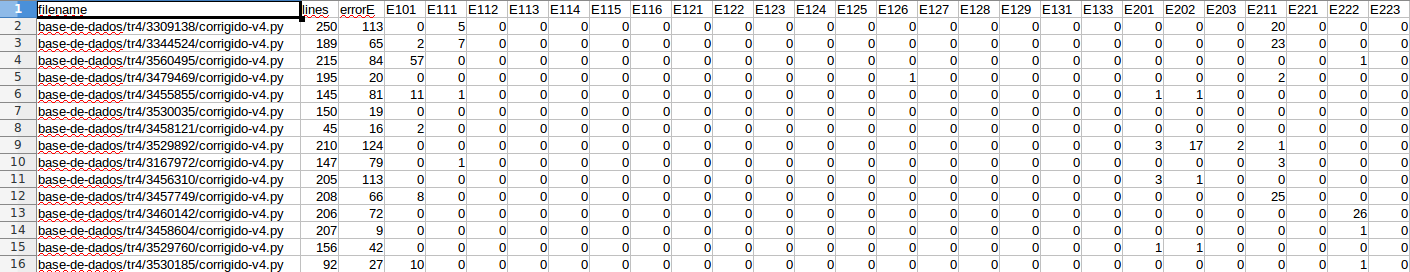
\includegraphics[width=1\linewidth]{imagem/arquivoCSV}
				\caption{Arquivo no formato \texttt{CSV} gerado após as adaptações inseridas nas ferramentas \texttt{Flake8} e \texttt{PEP8}}
				\label{fig:arquivoCSV}
			\end{figure}
			
			A \cref{fig:arquivoCSV} apresenta o arquivo gerado pelas ferramentas após a
			execução das análises de cada código-fonte presente no caminho \texttt{base-de-dados/}.
			As três primeiras colunas são: o nome do arquivo, a quantidade de linhas implementadas
			e o total de erros do estilo de escrita PEP 8 \cite{van2001pep}, respectivamente. As
			demais colunas são referentes a cada erro do \texttt{PEP8} \cite{pep8} com a última
			coluna representando a complexidade ciclomática calculada pela ferramenta
			\texttt{McCabe} \cite{mccabe}.


		\subsection{ScienceView}
		\label{sec:scienceView}
		
		A ferramenta \foreign{Science View} \cite{Alencar} foi desenvolvida para exibir
		as relações entre os documentos dado um acervo de artigos científicos, utilizando
		a \acs{T-LSP} a partir de artigos nos formatos \foreign{ISI}, \foreign{Endnote Export Format}
		ou \foreign{BibTeX}.

		A fim de criar uma nova projeção multidimensional dinâmica, a ferramenta guia o usuário
		para: inserir um novo conjunto de documentos ou utilizar uma coleção presente no banco
		de dados; definir parâmetros sobre o pré-processamentos dos dados e a redução de
		dimensionalidade; decidir qual ténica de projeção e o cálculo de distância a ser utilizado;
		e determinar os parâmetros referente a \acs{T-LSP}.

		% TODO: apresentar screenshot da tela de entrada (para importar a base gerada pela ScienceView-Python), da tela de normalização e da tela de projeção, com as devidas explicações. Mencione também, principalmente no início, as modificações que você fez na ferramenta (importação de dados no formato CSV, alteração do modelo de representação para valores em ponto flutuante e ajustes na ferramenta para calcular a projeção e os agrupamentos para este novo tipo de dados).

	\section{Considerações finais}
	
		O próximo capítulo % TODO: juntar aqui com o próximo parágrafo, indicando que o próximo capítulo descreve dois estudos sobre avaliação de programas em Python utilizando o método e as ferramentas apresentadas neste capítulo.
		As duas próximas seções irão descrever a visualização de duas bases de dados
		distintas, descrevendo a base de dados, sua avaliação, a forma que foi realizado
		seu experimento e o resultado qualitativo de cada uma.
\chapter{Resultados}
\label{chap:resultados}

	Neste capítulo, são apresentadas as avaliações da projeção e da visualização como
	instrumento para avaliação de programas, ambos considerando um conjunto de
	programas escritos em Python para uma disciplina introdutória à Computação.
	
	
	\section{Descrição da base}
	\label{sec:resultados:base-apoo}

		Essa base é constituída de 152 implementações em Python de 5 problemas distintos.
		Os desenvolvedores das implementações foram anonimizados, sendo representados por 
		sequências de números. Os problemas tratados foram os seguintes. O primeiro exercício
		consiste na revisão de conceitos básicos como: estruturas de condição e laço de repetição. O
		segundo exercício define a criação de classes com mais de um construtor, e manipulação de
		arquivos e cadeia de caracteres. O terceiro exercício consiste na criação das classes
		\texttt{Palavra} e \texttt{Texto}, no qual a primeira classe deve ser utilizada na segunda
		classe, e uma classe para gerar orações gramaticais. O quarto exercício refere-se a
		utilização de herança e polimorfismo, identificando cada palavra contida em um arquivo. O
		quinto exercício consiste na alteração de uma classe, implementando sobreposição de
		operadores. 
		
	
	\section{Avaliação da projeção com preservação de vizinhança}

		A \foreign{ScienceView} utiliza a preservação da vizinhança
		(\cref{subsubsec:vizinhanca}) para verificar a qualidade das projeções. A \cref{fig:neighborhoodAPOO30}
		apresenta a qualidade da projeção para essa base de dados. Essa técnica visa avaliar
		se houve uma preservação da vizinhança dos objetos no espaço de alta dimensionalidade
		na projeção. A \foreign{Neighborhood Preservation} é calculada tomando os $k$ vizinhos
		mais próximos de uma instância no espaço de alta dimensionalidade e os $k$ vizinhos
		mais próximos na projeção, e verificando-se que proporção da vizinhança é preservada
		na projeção. A precisão final para um dado valor de $k$ é a média das precisões para
		cada instância. Esse cálculo é feito para vários valores de $k$ (tipicamente $k=[2,...,30]$)
		de forma a obtermos uma curva. Quanto mais altos os valores da curva para cada valor
		de $k$, maior a qualidade da projeção. Considerando que a técnica \acl{T-LSP} \cite{Alencar}
		gera uma sequência de projeções, temos uma curva para cada projeção da
		sequência.
		
		Por exemplo, na \cref{fig:neighborhoodAPOO30} é possível observar que as projeções no início da
		sequência apresentam maior qualidade quando comparada as demais, como é possível observar
		nas curvas dos problemas 3, 4 e 5. Isso é esperado, dado que, além de serem considerados
		mais programas, os programas referentes aos problemas 3, 4 e 5 são mais complexos do que
		aqueles referentes aos problemas 1 e 2, com características mais diversificadas e difícil
		representação com precisão no espaço 2D da projeção. 
	
		\begin{figure}
			\centering
			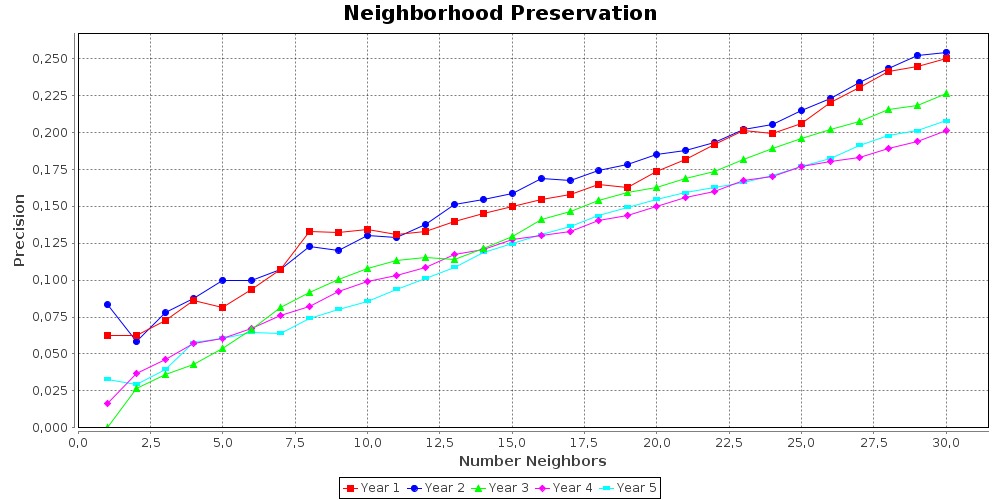
\includegraphics[width=0.85\linewidth]{imagem/neighborhoodAPOO30}
			\caption{Qualidade da projeção, utilizando a preservação de vizinhança (\foreign{neighborhood preservation})}
			\label{fig:neighborhoodAPOO30}
		\end{figure}	
	
		Finalmente, observa-se a precisão de 20\% para a linha (\texttt{year} $5$, obtida com 30 vizinhos para a
		projeção considerando todos os problemas (e, consequentemente, todas as submissões). Considerando
		outros trabalhos que utilizam esta medida para avaliação de qualidade de projeções~\cite{phd:paulovich},
		a qualidade da projeção é adequada e compatível com outras projeções feitas com a técnica LSP e
		similares.
		
		

	
	\section{Avaliação qualitativa da visualização}
	\label{sec:avalQualitativa}
	
		Para obter resultados qualitativos dessa pesquisa, realizamos um estudo experimental com
		as seguintes etapas: treinamento, utilização e questionário.
		
		% TODO: como foram organizadas as pessoas, quantas pessoas, os tempos
		
		O treinamento foi realizado na forma de tutorial com a apresentação dos critérios
		de avaliação (estilo de escrita e complexidade ciclomática) e da ferramenta com
		duração de $55$ minutos. Especificamente quanto à ferramenta, foram apresentados
		todos os passos referentes ao seu funcionamento, desde a inserção de uma nova
		coleção no banco de dados até a visualização das implementações com a visualização
		da projeção criada a partir da coleção. Em seguida, foi apresentado como utilizar
		a ferramenta para auxiliar na avaliação das implementações: visualizar os
		agrupamentos formados ao longo das projeções, selecionar um determinado conjunto
		de implementações, identificar as características semelhantes de tais grupos e
		abrir mais de uma implementação simultaneamente. Durante o treinamento, foi utilizada uma
		base de dados distinta da descrita na \cref{sec:resultados:base-apoo}.
		
		% TODO: informar que eles tiveram 20 minutos para avaliar trabalhos. 
		% TODO: falar quantas pessoas foram e como elas foram organizados (dois grupos: primeiramente, um grupo avaliou de forma tradicional, com auxílio dos dados obtidos pela ScienceView-Python e o outro grupo avaliou com auxílio da ferramenta. Depois foram invertidas as intervenções. Em ambos os casos, a cada rodada de avaliações, cada participante criou um relato sobre os programas avaliados e comentários que seriam enviados para os alunos, considerando os erros identificados.)
		Encerrado o treinamento, procedeu-se para a utilização da ferramenta com a base
		descrita na \cref{sec:resultados:base-apoo}. Para iniciarmos essa etapa, foi
		pedido para que os participantes encerrassem o funcionamento da \foreign{ScienceView}
		e a executassem com a criação da base de dados. O experimento teve participação
		de $4$ pessoas e ambos os grupos utilizaram os dados obtidos pela \foreign{ScienceView-Python}
		\cref{sec:scienceView-Python}. Todos os contribuintes realizaram  correção manual,
		o qual consistiu na correção somente do código-fonte sem utilizar a ferramenta, e
		somente $3$ pessoas utilizaram a ferramenta \foreign{ScienceView} para auxiliar
		na correção. O experimento consistiu em duas etapas. Na primeira etapa, $1$
		voluntário realizou a correção manual, enquanto os outros $2$, utilizaram a
		ferramenta para auxiliar na correção com duração de $20$ minutos. Na segunda
		etapa, o contribuinte que realizou a correção manual, passou a utilizar a
		\foreign{ScienceView}, enquanto os $2$ que utilizaram a ferramenta na etapa
		anterior, realizaram a correção manual durante $22$ minutos. Os participantes
		utilizaram a ferramenta sem ajuda no que já tinha sido apresentado e o
		avaliaram por meio de um questionário.		
		
		O questionário (\cref{apendice:questionario}) apresenta questões objetivas e
		dissertativas para avaliar a qualidade do treinamento e da ferramenta. Enquanto
		as questões objetivas visavam a qualidade do treinamento, da ferramenta e se
		é possível utilizá-la para auxiliar na correção, as questões dissertativas
		visam a encontrar lacunas observadas pelo participante para uma possível 
		atualização da ferramenta.
		
		A \cref{fig:projecaoFinal} apresenta a visualização dos agrupamentos das 152
		implementações contidas na base de dados. Isso foi possível após a adaptação da
		ferramenta para leitura de arquivos no formato \texttt{CSV}. Cada ponto da
		visualização é referente a um código-fonte. Ao clicar em um dos pontos,
		uma interface exibe sua implementação e as características extraídas pela
		\foreign{ScienceView-Python} para aquele código-fonte. Também é possível ordenar
		as colunas de características \foreign{Quantity} e \foreign{Normalized} em
		ordem  crescente ou decrescente para visualizar as características que mais
		ocorreram. Por padrão, a tabela é apresentado ordenada de forma decrescente
		pela coluna \foreign{Normalized}.
	
		\begin{figure}[h]
			\centering
			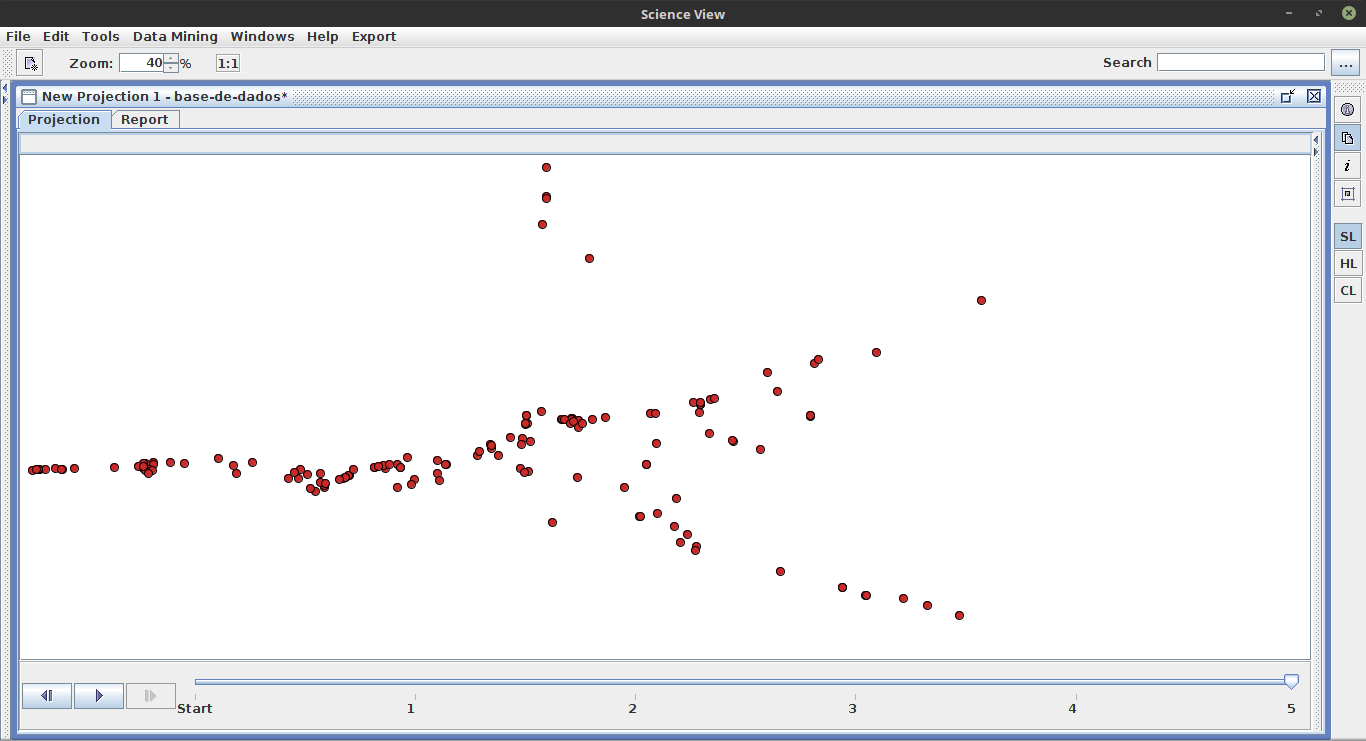
\includegraphics[width=1\linewidth]{imagem/projecaoFinal} % TODO: substituir, futuramente, pela figura da ferramenta corrigida.
			\caption[Visualização dos agrupamentos da base de dados gerado pela \texttt{ScienceView}]
			{Visualização dos agrupamentos da base de dados gerado pela \texttt{ScienceView} \cite{Alencar-etal:2012}}
			\label{fig:projecaoFinal}
		\end{figure}
		
		A \cref{tab:resultados} apresenta a quantidade de implementações que cada
		participante corrigiu e de comentários realizados. A primeira linha identifica
		qual participante realizou as correções. E a primeira coluna indica a forma
		de correção realizada pelos voluntários. Então, é apresentado a quantidade
		de correções que cada participante conseguiu realizar e a quantidade de
		comentários conforme o tipo de correção.
		
		\begin{table}[h]
			\begin{tabularx}{\linewidth}{|X|X|X|X|X|}
		        \hline
		        
		        & Voluntário 1
		        & Voluntário 2
		        & Voluntário 3
		        & Voluntário 4\\
		        
		        \hline
		        Correção tradicional
		        & 3 códigos-fontes e 2 comentários para correção do aluno
		        & 4 códigos-fontes e 3 comentários para correção do aluno
		        & 3 códigos-fontes e 2 comentários para correção do aluno
		        & 5 códigos-fontes e 2 comentários para correção do aluno\\
		        
		        \hline
		        \foreign{ScienceView}
		        & Não utilizou a ferramenta
		        & 4 códigos-fontes e 4 comentários realizados
		        & 3 códigos-fontes e observou que a ferramenta auxiliou no encontro dos erros de forma mais rápida.
		        & 4 códigos-fontes e 3 comentários para correção dos alunos\\
		        \hline
			\end{tabularx}
			\caption{Quantidade de correções e comentários realizados com e sem a utilização da ferramenta}
			\label{tab:resultados}
		\end{table}
		
%		As implementações das \cref{fig:codigo1} e \cref{fig:codigo2} foram consideradas
%		semelhantes, devido aos seus respectivos pontos estarem próximos no mapa de
%		projeção. É possível notar que há diversas semelhanças nos tipos das características
%		extraídas e erros que ocorreram pela coluna \foreign{Normalized}, além da quantidade
%		dessas características apresentadas na coluna \foreign{Quantity}.
%		
%		\begin{figure}[h]
%			\centering
%			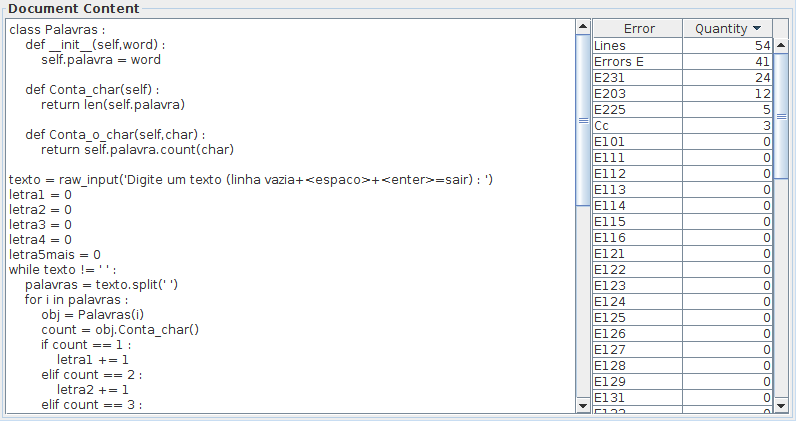
\includegraphics[width=0.8\linewidth]{imagem/codigo1}
%			\caption[Representação parcial da interface que apresenta o código e suas características]
%			{Representação parcial da interface que apresenta o código e suas características \cite{Alencar-etal:2012}}
%			\label{fig:codigo1}
%		\end{figure}
%		
%		\begin{figure}[H]
%			\centering
%			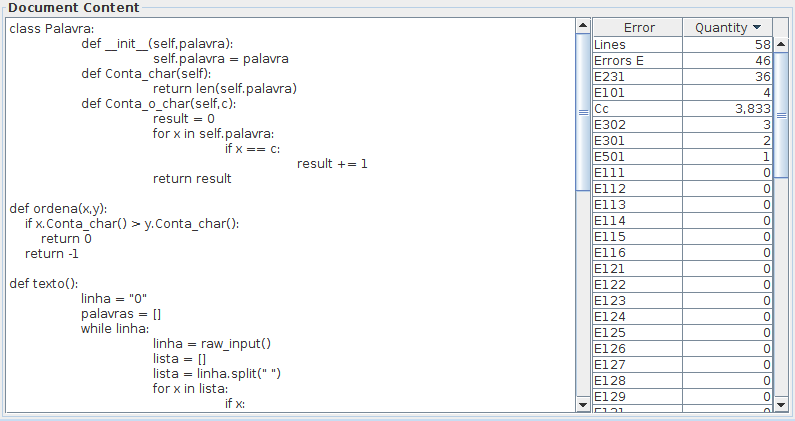
\includegraphics[width=0.8\linewidth]{imagem/codigo2}
%			\caption[Representação parcial da interface que apresenta o código considerado semelhante ao da \cref{fig:codigo1}]
%			{Representação parcial da interface que apresenta o código considerado semelhante ao da \cref{fig:codigo1} \cite{Alencar-etal:2012}}
%			\label{fig:codigo2}
%		\end{figure}
		
		Para finalizar o experimentos, os voluntários, responderam o questionário (\cref{apendice:questionario})
		anonimamente. A primeira questão refere-se ao tempo de experiência como professor,
		visto que acreditávamos que essa experiência poderia interferir na quantidade
		de correções realizadas com a ferramenta. Dentre eles, $2$ cooperadores possuem
		menos que $1$ ano de experiência, enquanto $1$ possui mais de $10$ anos de
		experiência como professor. E todos eles afirmaram que o treinamento em forma
		de tutorial da \foreign{ScienceView} contribui para sua utilização.
		
		Obtivemos êxito com a adaptação da interface que apresenta o código-fonte e a
		tabela de erros, visto que, ao serem questionados se faltava
		alguma informação nessa interface, todos responderam negativamente.
		
		Apesar dos $3$ voluntários afirmarem que a \foreign{ScienceView} colaborou
		para a correção das implementações, $2$ deles corrigiram a mesma quantidade
		de implementações utilizando a ferramenta e manualmente. A exceção ocorreu com 
		apenas $1$ participante que extraiu os tópicos semelhantes manualmente. Na
		primeira extração, selecionou apenas $2$ códigos-fontes e observou que os
		erros apresentados na tabela de erros eram semelhantes, visto que observou
		a importação de bibliotecas entre funções ao invés de realizá-las no início
		da implementação. Na segunda extração, selecionou $8$ códigos-fontes e constatou
		que os erros ocorreram nas implementações e foi compreendido corretamente
		pela ferramenta.
		
		Ao relatarem sobre o \foreign{feedback} recebido da \foreign{ScienceView}
		por meio da visualização dos agrupamentos, $2$ participantes afirmaram que
		os agrupamentos auxiliaram na verificação de implementações com características
		similares. O outro participantes constatou a possibilidade de utilizar a
		ferramenta em uma turma fechada de alunos a fim de verificar quais os principais
		erros deles por meio da extração de tópicos da ferramenta.
		
		Sobre a experiência em relação ao uso da ferramenta, um dos participantes
		admite que, como não utilizou muito a ferramenta, foi mais rápido realizar
		as correções manuais. Contudo, outra resposta afirma que a utilização mais
		frequente da \foreign{ScienceView}, evidenciará analisar as implementações
		de forma mais rápida.
		
		
% TODO: deixar para artigo
%	
%	\section{Projeção e visualização de MIT 6.00.1x}	
%
%	\subsection{Descrição da base}
%	% TODO: descrever base de dados: quais foram os tipos de programas, quantos foram, falar que a
%	% base não foi anonimizada porque os programas estavam publicamente disponíveis no GitHub.
%	Essa base de dados é constituída de 3470 implementações referente a 10 exercícios
%	distintos. Todos as atividades solicitam manipulação de arquivo e cadeia de caracteres.
%	
%	O primeiro exercício requer conceitos de matriz, utilizando lista dentro
%	de lista, e programação dinâmica para solucionar o transporte de animais.
%	
%	O segundo exercício necessita de conhecimento sobre aleatoriedade, lista, condicional,
%	cadeia de caracteres, operações aritméticas e lógicas para implementar o jogo da
%	forca.
%	
%	O terceiro exercício solicita a utilização de laço de repetição, condicional, lista,
%	operações aritméticas e lógicas para implementar o jogo das palavras.
%	
%	O quarto exercício requer conhecimento de lista e dicionário pra codificar e
%	decodificar um texto.
%	O quinto exercício requer o uso de analisador (\foreign{parser}), construção
%	de classe, interface, polimorfismo e operadores lógicos para desenvolver um programa
%	de monitoramento de novos \foreign{feeds} na Internet.
%	
%	O sexto exercício solicita conhecimento sobre criação de classes, matriz, laço de
%	repetição e manipulação de interface gráfica para implementar um aspirador de pó
%	inteligente e sua simulação.
%	
%	O sétimo exercício consiste no uso de classes, aleatoriedade, laço de repetição,
%	condicional, lista e conhecimento de estatística para implementar uma simulação
%	e um sistema de tratamento de pacientes conforme o vírus que eles possuem.
%	
%	O oitavo problema consiste na implementação de classes a partir do exercício $7$.
%	Pedindo a implementação da classe \texttt{ResistantVirus} e \texttt{SimplePatient}
%	para realizar simulações desses vírus em pacientes.
%	
%	O nono exercício requer o uso de dicionário e operador lógico para desenvolver
%	um software que apresente uma lista de assuntos para cada aluno da universidade.
%	
%	E para o décimo exercício, é necessário conhecer um algoritmo de agrupamento para
%	realizar sua implementação.
%	
%	Os desenvolvedores dessas implementações não foram anonimizados, pois seus
%	códigos-fontes estavam presentes em repositórios públicos no GitHub \cite{github}.
%	
%	% TODO: Marco: colocar a string utilizada para buscar os programas e como foi criada a base
%	
%
%\subsection{Avaliação da projeção com preservação de vizinhança}
%
%
%\subsection{Avaliação qualitativa da visualização}
%% TODO: relatar o estudo: treinamento, instruções, questionário, resultados

	\section{Ameaças a validade}
	\label{sec:ameacas}
	
		% TODO: treinamento não foi suficiente para utilização da ferramenta para avaliação
		O treinamento realizado, não foi suficiente para avaliar as implementações por meio
		da utilização da \foreign{ScienceView}, visto que um dos participantes relatou que
		a falta de conhecimento sobre a ferramenta fez com que correção manual acontecesse de
		forma mais rápida. Enquanto, outro participante observou que a ferramenta agilizará
		o processo de correção conforme aumentar a frequência de uso da ferramenta. Dado
		essas duas observações, podemos concluir que o treinamento não foi suficiente para
		capacitar todos os participantes sobre a utilização da ferramenta.
		
		% TODO: treinamento tem de deixar claro que a avaliação é quanto aos trabalhos, mas não quanto a correção dos problemas automaticamente identicados
		Durante o treinamento, não foi exposto explicitamente que, ao utilizar a \foreign{ScienceView},
		a avaliação é quanto aos códigos-fontes. Com isso, além de corrigirem as implementações,
		alguns participantes buscaram verificar se as características semelhantes apontadas
		pela extração de tópicos realmente ocorria nas implementações. E isso pode ter
		impactado na correção, devido ao tempo gasto para fazer essas verificações.
		
		% TODO: outra ameaça é quanto ao tamanho da base
		O banco de dados formado por 152 códigos-fontes que solucionam 5 problemas distintos
		é considerado pequeno. Visto que, uma das características do \ac{MOOC} é a grande
		quantidade de usuários (\foreign{massive}). Desta forma, essa base de dados não
		reflete ao montante de submissões que podem ocorrer em um \acs{MOOC}
		
		% TODO: outra ameaça é quanto a quantidade de participantes
		A aplicação do experimento somente com $4$ pessoas, e ainda, somente $3$ pessoas
		utilizarem a \foreign{ScienceView} não nos retorna nada concreto estatisticamente.
		Devido a essa quantidade, temos apenas indícios do objetivo da pesquisa. Para
		viabilizar mais participantes, é necessário, além de tempo, a disponibilidade
		de professores para participar do treinamento e utilizar a ferramenta, focando
		que o desenvolvimento do projeto pode contribuir para vossas correções, além
		de possibilitar a verificação do erro mais frequente a fim de melhorar suas
		aulas.

	\section{Considerações finais}
	
		Por meio dos resultados obtidos, a próxima Seção apresentará nossa conclusão,
		considerando tanto a análise qualitativa, quanto a quantitativa. E as ameaças
		a validade observadas.

\chapter{Conclusão}
\label{chap:Conclusao}

	Este capítulo apresenta nossa conclusão com base nos resultados obtidos a fim de
	responder nossas questões de pesquisa e os trabalhos futuros para uma possível
	continuidade do projeto.
	
	Por meio dos resultados obtidos, podemos responder nossas questões de pesquisa
	firmadas na \cref{sec:metodo}:
	
	\begin{itemize}
		\item \textbf{QP$_1$}: o algoritmo de agrupamento produz grupos de códigos-fontes
		com boa qualidade?
		\item \textbf{QP$_2$}: a utilização de subsídios de avaliação reduz o tempo
		de correção de todas as submissões?
	\end{itemize}
	
	A fim de responder a \textbf{QP$_1$}, foi estudado e utilizado a preservação
	da vizinhança \cite{paulovich2008hipp}, que quantifica a qualidade de uma projeção.
	Sua utilização ocorreu por meio da \foreign{ScienceView}. Tomaremos, como base
	para a nossa resposta, a \cref{fig:neighborhoodAPOO30}. Considerando outros trabalhos
	que utilizam esta medida para avaliação de qualidade de projeções~\cite{phd:paulovich},
	a qualidade da projeção é adequada e compatível com outras projeções feitas com
	a técnica LSP e similares, visto que obteve resultado semelhante aos obtidos por
	\citeonline{phd:paulovich}.
% Por meio dela é possível
%	observar que, quanto maior a quantidade de dados a serem observados, menor a perca
%	na qualidade da projeção.
%	As variações que ocorrem nas curvas vermelha e azul
%	escuro, na instância de tempo $1$ e $2$, respectivamente, possuem perca de
%	qualidade maior quando comparadas com as curvas rosa e azul claro, na instância de
%	tempo $4$ e $5$, respectivamente. Desta forma, responderemos a questão de pesquisa
%	a seguir, utilizando as curvas das instâncias de tempo $4$ e $5$.
%	O algoritmo de agrupamentos gera grupos com boa qualidade, com precisão de $20\%$
%	quando consideramos a quantidade de vizinhos
%	igual a $30$. No melhor caso, ocorre uma perca de aproximadamente $12,5\%$ quando
%	a quantidade de vizinhos é igual a $15$. Desta forma, entre $15$ vizinhos de um
%	código-fonte qualquer, no máximo duas implementações estão agrupadas inadequadamente. 
	
	Para responder a \textbf{QP$_2$} foi necessário aplicar o estudo
	para saber quantas implementações os participantes analisariam em um determinado
	período de tempo, realizando as correções manualmente e por meio da utilização dos
	subsídios proposto. A utilização de subsídios não reduziu o tempo de correção
	das implementações em um período de $20$ minutos, visto que alguns participantes
	corrigiram a mesma quantidade de implementações nas duas formas de análise, enquanto
	um participante realizou mais correções manualmente, quando comparado a utilização
	da ferramenta.

	Contudo, quando utilizaram a \foreign{ScienceView}, podemos observar
	que os participantes realizaram poucas correções de implementações que estão no
	mesmo agrupamento. O Voluntário 2 (\cref{tab:resultados}) analisou uma implementação
	de um agrupamento com 9 códigos-fontes, duas implementações de um grupo com 12
	códigos-fontes e uma implementação de um agrupamento contendo 5 códigos-fontes
	distintos. O Voluntário 3, apesar de corrigir uma implementação que estava isolada
	na projeção, analisou uma implementação de um agrupamento contendo 12 códigos-fontes
	e uma implementação de um agrupamento com 8 códigos-fontes. Finalmente, o Voluntário 4
	corrigiu uma implementação que estava isolada na projeção, uma implementação de
	um agrupamento contendo 5 códigos-fontes, e duas implementação de agrupamentos
	distintos contendo 2 códigos-fontes distintos. Apesar de não podermos comprovar
	a segunda questão de pesquisa, o total de códigos-fontes que podem ser considerados
	corrigidos por meio da correção de uma implementação do agrupamento é alta. Isso
	nos dá indícios que, se melhorarmos	o treinamento, poderemos alcançar nosso objetivo.
	
%	A negativa para essa resposta pode ser pela pouca experiência de uso
%	com a \foreign{ScienceView}, como também a preocupação de alguns participantes em
%	verificar se os erros apresentados na extração de tópicos realmente aconteceram
%	nas implementações.
	
	Como trabalhos futuros, é importante sanar as ameaças a validade (\cref{sec:ameacas})
	desse projeto. Focando, inicialmente, na construção de uma base de dados de
	implementações maior, a fim de tornar-se próximo a quantidade de submissões
	possíveis em um \acs{MOOC}. Em seguida, melhorar nosso treinamento para que
	todos os participantes utilizem a ferramenta para sua finalidade, e encontrar
	mais professores dispostos a participar de todo o experimento.
	
	Para uma base de dados maior, seria interessante avaliar o quanto as características
	extraídas neste estudo são relevantes e, caso necessário, realimentar o
	sistema da mineração de dados, como descrito na \cref{sec:FundTeor}. Por
	exemplo, poderia-se considerar características dinâmicas das submissões, executando
	casos de teste e, encontrando as variáveis
	comuns e renomeando-as para o nome mais utilizado \cite{Glassman:2015}.
	A combinação da análise dinâmica e estática pode gerar resultados melhores e
	particularmente úteis para avaliação de programas.


\bibliographystyle{abntex2-alf}
\bibliography{main}

\backmatter
\appendix
\chapter{Erros do PEP8}
\label{apendice:pep8}

	\begin{table}
		\scriptsize
		\begin{tabularx}{\linewidth}{ |l|X|X| }
			\hline
			\textbf{Erro}
			& \textbf{Descrição}
			& \textbf{Exemplo do erro} \\
			\hline
			
			&
			& Correto: if a == 0:$\backslash$n \ \ \ \ a = 1$\backslash$n \ \ \ \ b = 1 \\
			\hline
			E101
			& Indentação contém espaços e tabulações misturados
			& if a == 0:$\backslash$n \ \ \ \ a = 1$\backslash$n$\backslash$tb = 1 \\
			\hline
			
			&
			&  \\
			\hline
			
			&
			& Correto: a = 1 ou if a == 0:$\backslash$n \ \ \ \ a = 1 \\
			\hline
			E111
			& Nível sem indentação e foi encontrado espaços em branco
			&  \\
			\hline
			E112
			& Nível com uma indentação, mas não foi encontrado uma indentação
			&  \\
			\hline
			E113
			& Nível sem indentação e foi encontrado indentação
			&  \\
			\hline
			E114
			& Nível sem indentação e foi encontrado espaços em branco e comentário de uma linha
			&  \\
			\hline
			E115
			& Nível com uma indentação, mas não foi encontrado uma indentação, seguido de comentário
			&  \\
			\hline
			E116
			& Nível sem indentação e foi encontrado indentação seguido de comentário
			&  \\
			\hline
			
			&  
			&  \\
			\hline
			
			&
			& Correto: a = ($\backslash$n) ou a = ($\backslash$n \ \ \ \ 42) \\
			\hline
			E121
			& Há espaços, porém é menos que uma tabulação (4 espaços)
			& a = ($\backslash$n   42) \\
			\hline
			E122
			& Sem indentação
			& a = ($\backslash$n42) \\
			\hline
			E123
			& Não encontra ")" ou indentation of opening bracket's line
			& a = ($\backslash$n \ \ \ \ ) ou a = ($\backslash$n \ \ \ \ 42$\backslash$n \ \ \ \ ) \\
			\hline
			E124
			& Não encontra ")" visualmente indentado
			& a = (24,$\backslash$n \ \ \ \  42$\backslash$n) \\
			\hline
			E125
			& Falta indentação na continuação da declaração
			& if ($\backslash$n \ \ \ \ b):$\backslash$n \ \ \ \ pass \\
			\hline
			E126
			& Excesso de indentação para ")"
			& a = ($\backslash$n \ \ \ \ 42) \\
			\hline
			E127
			& Excesso de indentação afim de indentar visualmente
			& a = (24,$\backslash$n \ \ \ \   42) \\
			\hline
			E128
			& Continuação da linha com limitação de indentação para indentar visualmente
			& a = (24,$\backslash$n \ \ \ \ 42) \\
			\hline
			E129
			& Linha indentada visualmente
			& if (a or$\backslash$n \ \ \ \ b):$\backslash$n \ \ \ \ pass \\
			\hline
			E131
			& unaligned for hanging indent
			& a = ($\backslash$n \ \ \ \ 42$\backslash$n 24) \\
			\hline
			E133
			& Fecha ")" e falta indentação
			&  \\
			\hline
		\end{tabularx}
		\caption{Erros extraídos do estilo de escrita PEP8 referente a indentação}
		\label{tab:pep8E100}
	\end{table}

	\begin{table}
		\tiny
		\begin{tabularx}{\linewidth}{ |l|X|X| }
			\hline
			\textbf{Erro}
			& \textbf{Descrição}
			& \textbf{Exemplo do erro} \\
			\hline
			
			& 
			& Correto: spam(ham[1], \{eggs: 2\}) \\ 
			\hline
			E201 
			& Espaço em branco após (, [ ou \{ 
			& spam( ham[1], \{eggs: 2\}) \\ 
			\hline
			E202 
			& Espaço em branco antes de ), ] ou   
			& spam(ham[1], \{eggs: 2\} ) \\ 
			\hline
			E203 
			& Espaço em branco antes de ":", ";", "," 
			& if x == 4: print x, y; x, y = y , x \\ 
			\hline
			
			& 
			&  \\ 
			\hline
			
			& 
			& Correto: spam(1) ou dict['key'] = list[index] \\ 
			\hline
			E211 
			& Espaço em branco antes de "(" ou "[" 
			& dict ['key'] = list[index] ou dict['key'] = list [index] \\ 
			\hline
			
			& 
			&  \\ 
			\hline
			
			& 
			& Correto: a = 12 + 3 \\ 
			\hline
			E221 
			& Múltiplos espaços antes do operador 
			& a = 4  + 5 \\ 
			\hline
			E222 
			& Múltiplos espaços depois do operador 
			& a = 4 +  5 \\ 
			\hline
			E223 
			& Tabulação antes do operador 
			& a = 4$\backslash$t+ 5 \\ 
			\hline
			E224 
			& Tabulação depois do operador 
			& a = 4 +$\backslash$t5 \\ 
			\hline
			
			& 
			&  \\ 
			\hline
			
			& 
			& Correto: foo(bar, key='word', *args, **kwargs) \\ 
			\hline
			E225 
			& Falta espaço em branco em volta do operador 
			& i=i+1 \\ 
			\hline
			E226 
			& Aritmética 
			& c = (a+b) * (a-b) ou hypot2 = x*x + y*y \\ 
			\hline
			E227 
			& Bit a bit ou shift 
			& c = a|b \\ 
			\hline
			E228 
			& Modulo 
			& msg = fmt\%(errno, errmsg) \\ 
			\hline
			
			& 
			&  \\ 
			\hline
			
			& 
			& Correto: [a, b] ou (3,) ou a[1:4] ou a[1:4:2] \\ 
			\hline
			E231 
			& Não tem espaço em branco após ",", ";" e ":" 
			& ['a','b'] \\ 
			\hline
			
			& 
			&  \\ 
			\hline
			
			& 
			& Correto: a = (1, 2) \\ 
			\hline
			E241 
			& Múltiplos espaços após "," 
			& a = (1,  2) \\ 
			\hline
			E242 
			& Tabulação após "," 
			& a = (1,$\backslash$t2) \\ 
			\hline
			
			& 
			&  \\ 
			\hline
			
			& 
			& Correto: def complex(real, imag=0.0): ou boolean(a >= b) \\ 
			\hline
			E251 
			& Espaços inesperados ao redor de "=" (atribuição) 
			& def complex(real, imag = 0.0): \\ 
			\hline
			
			& 
			&  \\ 
			\hline
			
			& 
			& Correto: x = x + 1  \# Increment x ou x = x + 1 \ \ \ \ \# Increment x \\ 
			\hline
			E261 
			& Menos de dois espaços antes do comentário 
			& x = x + 1 \# Increment x \\ 
			\hline
			E262 
			& Comentário deve iniciar com \# e um espaço 
			& x = x + 1  \#Increment x ou x = x + 1  \#  Increment x \\ 
			\hline
			E265 
			& Comentário em bloco deve inicar com \# e um espaço 
			& \#Block comment \\ 
			\hline
			E266 
			& Muitos \# para o bloco de comentário 
			& \#\#\# Block comment \\ 
			\hline
			
			& 
			&  \\ 
			\hline
			
			& 
			& Correto: True and False \\ 
			\hline
			E271 
			& Múltiplos espaços antes de uma palavra reservada
			& True and  False \\ 
			\hline
			E272 
			& Múltiplos espaços depois de uma palavra reservada 
			& True  and False \\ 
			\hline
			E273 
			& Tabulação após a palavra reservada 
			& True and$\backslash$tFalse \\ 
			\hline
			E274 
			& Tabulação antes da palavra reservada 
			& True$\backslash$tand False \\ 
			\hline
		\end{tabularx}
		\caption{Erros extraídos do estilo de escrita PEP8 referente a espaços em branco}
		\label{tab:pep8E200}
	\end{table}

	\begin{table}
		\scriptsize
		\begin{tabularx}{\linewidth}{ |l|X|X| }
			\hline
			\textbf{Erro}
			& \textbf{Descrição}
			& \textbf{Exemplo do erro} \\
			\hline
			
			& 
			& Correto: def a():$\backslash$n \ \ \ \ pass$\backslash$n$\backslash$n$\backslash$ndef b():$\backslash$n \ \ \ \ pass \\ 
			\hline
			
			& 
			& Correto: def a():$\backslash$n \ \ \ \ pass$\backslash$n$\backslash$n$\backslash$n\# Foo$\backslash$n\# Bar$\backslash$n$\backslash$ndef b():$\backslash$n \ \ \ \ pass \\ 
			\hline
			E301 
			& Espera uma linha em branco e encontrou nenhuma 
			& class Foo:$\backslash$n \ \ \ \ b = 0$\backslash$n \ \ \ \ def bar():$\backslash$n \ \ \ \  \ \ \ \ pass \\ 
			\hline
			E302 
			& Espera duas linhas em branco e encontrou uma quantidade diferente de dois 
			& def a():$\backslash$n \ \ \ \ pass$\backslash$n$\backslash$ndef b(n):$\backslash$n \ \ \ \ pass \\ 
			\hline
			E303 
			& Muitas linhas em branco 
			& def a():$\backslash$n \ \ \ \ pass$\backslash$n$\backslash$n$\backslash$n$\backslash$ndef b(n):$\backslash$n \ \ \ \ pass \\ 
			\hline
			E304 
			& Blank lines found after function decorator - Encontrou linhas em branco após a função principal 
			& @decorator$\backslash$n$\backslash$ndef a():$\backslash$n \ \ \ \ pass \\ 
			\hline
		\end{tabularx}
		\caption{Erros extraídos do estilo de escrita PEP8 referente a linhas em branco}
		\label{tab:pep8E300}
	\end{table}

	\begin{table}
		\scriptsize
		\begin{tabularx}{\linewidth}{ |l|X|X| }
			\hline
			\textbf{Erro}
			& \textbf{Descrição}
			& \textbf{Exemplo do erro} \\
			\hline
			
			& 
			& Correto: import os$\backslash$nimport sys \\ 
			\hline
			E401 
			& Múltiplos import em uma linha 
			& import sys, os \\ 
			\hline
		\end{tabularx}
		\caption{Erros extraídos do estilo de escrita PEP8 referente a importação de bibliotecas}
		\label{tab:pep8E400}
	\end{table}

	\begin{table}
		\scriptsize
		\begin{tabularx}{\linewidth}{ |l|X|X| }
			\hline
			\textbf{Erro}
			& \textbf{Descrição}
			& \textbf{Exemplo do erro} \\
			\hline
			E501 
			& Linha com 80 caractéres ou mais 
			& Correto: aaa = [123,$\backslash$n \ \ \ \ \ \ \ \  \ \ \ \ \ \ \ \ 123] \\
			\hline
			& 
			& Correto: aaa = ("bbb "$\backslash$n \ \ \ \ \ \ \ \  \ \ \ \ \ \ \ \ "ccc") \\
			\hline
			& 
			& Correto: aaa = "bbb " $\backslash$$\backslash$n \ \ \ \ \ \ \ \ "ccc" \\
			\hline
			& 
			& Correto: aaa = 123  \# $\backslash$$\backslash$ \\
			\hline
			& 
			&  \\
			\hline
			E502 
			& Contrabarra é redundante entre parênteses 
			& aaa = [123, $\backslash$$\backslash$n \ \ \ \ \ \ \ \  \ \ \ \ \ \ \ \ 123] ou aaa = ("bbb " $\backslash$$\backslash$n \ \ \ \ \ \ \ \  \ \ \ \ \ \ \ \ "ccc") \\
			\hline
		\end{tabularx}
		\caption{Erros extraídos do estilo de escrita PEP8 referente a tamanho da instrução em caracteres}
		\label{tab:pep8E500}
	\end{table}

	\begin{table}
		\scriptsize
		\begin{tabularx}{\linewidth}{ |l|X|X| }
			\hline
			\textbf{Erro}
			& \textbf{Descrição}
			& \textbf{Exemplo do erro} \\
			\hline
			
			& 
			& Correto: if foo == 'blah':$\backslash$n \ \ \ \ do\_blah\_thing() \\
			\hline
			
			& 
			& Correto: do\_one() ou do\_two() ou do\_three() \\
			\hline
			E701 
			& Várias instruções em uma linha com ":" 
			& if foo == 'blah': do\_blah\_thing() \\
			\hline
			E702 
			& Múltiplas instruções em uma linha separados com ";" 
			& do\_one(); do\_two(); do\_three() \\
			\hline
			E703 
			& Declaração termina com um ";" 
			& do\_four();  \# useless semicolon \\
			\hline
			
			& 
			&  \\
			\hline
			
			& 
			& Correto: if arg is not None: \\
			\hline
			E711 
			& Comparar singleton com com operador lógico diferente
			& if arg != None: \\
			\hline
			E712 
			& Comparar singleton com com operador lógico igual
			& if arg == True: \\
			\hline
			
			& 
			&  \\
			\hline
			
			& 
			& Correto: if x not in y:$\backslash$n \ \ \ \ pass \\
			\hline
			
			& 
			& Correto: assert (X in Y or X is Z) \\
			\hline
			
			& 
			& Correto: if not (X in Y):$\backslash$n    pass \\
			\hline
			
			& 
			& Correto: zz = x is not y \\
			\hline
			E713 
			& Deve-se utilizar not in para verificar se variável está contido em outra 
			& Z = not X in Y ou if not X.B in Y:$\backslash$n \ \ \ \ pass \\
			\hline
			E714 
			& Deve-se utilizar is not para comparar objeto 
			& if not X is Y:$\backslash$n \ \ \ \ pass ou Z = not X.B is Y \\
			\hline
			
			& 
			&  \\
			\hline
			
			& 
			& Correto: if isinstance(obj, int): \\
			\hline
			E721 
			& Não comparar tipos, usar isinstance() 
			& if type(obj) is type(1): \\
			\hline
		\end{tabularx}
		\caption{Erros extraídos do estilo de escrita PEP8 referente a quantidade de instrução por linha e formas de instrução}
		\label{tab:pep8E700}
	\end{table}

	\begin{table}
		\scriptsize
		\begin{tabularx}{\linewidth}{ |l|X|X| }
			\hline
			\textbf{Erro}
			& \textbf{Descrição}
			& \textbf{Exemplo do erro} \\
			\hline
			E901 
			& Checa se a sintaxe é válida 
			&  \\
			\hline
			E902 
			& Tokenize the file, run physical line checks and yield tokens 
			&  \\
			\hline
		\end{tabularx}
		\caption{Erros extraídos do estilo de escrita PEP8 referente a verificação de sintaxe e geração de \foreign{tokens}}
		\label{tab:pep8E900}
	\end{table}
\begin{enumerate}
	\item O tutorial ajudou a utilizar a ferramenta?
	\item Caso a resposta anterior for negativa, quais informações podem ser apresentadas no tutorial?
	
	\item A descrição do exercício estava bem detalhada para solucionar o problema? (Sim ou Não)
	\item A descrição do exercício ocasionou dúvidas em relação ao desenvolvimento da solução? (Sim ou Não)
	\item Faltou alguma informação a ser apresentada na janela que consta o código-fonte?
	\item Em relação a pergunta anterior. Se respondeu "Sim", quais informações podem ser apresentadas?
	
	\item A visualização da projeção na Science View, colaborou para a correção das implementações?
	\item Disserte sobre o feedback recebido da Science View por meio da visualização dos agrupamentos.
	\item Disserte sobre a sua experiência em relação ao uso da Science View.
	
	Professor, em relação as perguntas da descrição do exercício, acredito que a primeira esteja induzindo a resposta. Por isso fiz a segunda. Achei importante perguntar sobre a descrição, porque pode ocorrer erros de implementação no caso de dúvidas gerados a partir do enunciado do exercício.
	
	Em relação a ultima questão, fiz para tentar capturar algumas características que não é possível obter pela escala Likert.
\end{enumerate}

\end{document}
